% ----------------------------------------------------------
% 6. Projeto de Interação
% ----------------------------------------------------------
\chapter{Projeto de Interação}
\label{cap:interacao}

Link para o Projeto de Interação do Sistema no Figma (compartilhado com a professora):

\noindent\url{https://www.figma.com/design/DR6oCNn8QeMXILJPJx4L4D/Sem-t%C3%ADtulo?node-id=0-1&p=f&t=UNW3lNd1nkxwVpfd-0}

Abaixo são apresentados os protótipos das telas de interface elaborados no Figma, estruturados conforme os casos de uso do Diagrama de Casos de Uso (Seção~\ref{cap:requisitos}). A Tabela~\ref{tab:rastreabilidade} relaciona cada caso de uso às telas que o realizam.

\section{Observações para o teste do protótipo}

O protótipo possui \textbf{6 fluxos principais}. Sugere-se testá-los na ordem abaixo, pois ela segue o ciclo de uso típico do sistema:

\begin{enumerate}
    \item \textbf{Membro e contestação} (PT-001, 002, 003, 016, 017, 018): login, consulta do perfil e das penalidades e envio de uma contestação.
    \item \textbf{Gestão de Pessoas} (PT-004 a 006, 008, 015): cadastro, edição e desligamento de membros, termos jurídicos e julgamento da contestação enviada no fluxo 1.
    \item \textbf{Horas de extensão} (PT-009, 010, 011): regras por cargo, contabilização e envio ao professor orientador.
    \item \textbf{Gerente} (PT-012 a 014, 026 a 032): registro de ocorrência disciplinar, projetos e tarefas e funil comercial.
    \item \textbf{Comunicação e agenda} (PT-007, 019 a 023): diretório, publicação de aviso e agendamento de eventos e reuniões 1-on-1.
    \item \textbf{Diretoria e finanças} (PT-024, 025, 033 a 035): propostas de governança, votação, lançamentos financeiros e aprovação de reembolsos.
\end{enumerate}
% VERIFICAR: confirmar no Figma se os fluxos acima estão ligados (clicáveis) na ordem descrita.

\section{Rastreabilidade entre casos de uso e telas}

\begin{center}
\footnotesize
\begin{longtable}{|c|p{5.2cm}|p{5.6cm}|}
\caption{Casos de uso e telas do protótipo}\label{tab:rastreabilidade}\\
\hline
\textbf{Caso de uso} & \textbf{Nome} & \textbf{Telas} \\
\hline
\endfirsthead
\hline
\textbf{Caso de uso} & \textbf{Nome} & \textbf{Telas} \\
\hline
\endhead
UC-01 & Autenticar-se & PT-001, PT-002 \\ \hline
UC-02 & Consultar meu perfil & PT-003, PT-016 \\ \hline
UC-03 & Consultar diretório da equipe & PT-007 \\ \hline
UC-04 & Consultar quadro de avisos & \textbf{(sem tela -- ver pendências)} \\ \hline
UC-05 & Gerenciar calendário & PT-020 a PT-023 \\ \hline
UC-06 & Contestar ocorrência & PT-016, PT-017, PT-018 \\ \hline
UC-07 & Consultar projetos e tarefas & PT-028, PT-029 \\ \hline
UC-08 & Gerenciar documentos e termos & PT-008 \\ \hline
UC-09 & Gerenciar cadastro de membros & PT-004, PT-005, PT-006 \\ \hline
UC-10 & Publicar aviso & PT-019 \\ \hline
UC-11 & Julgar contestação & PT-015 \\ \hline
UC-12 & Parametrizar regras de horas & PT-009 \\ \hline
UC-13 & Contabilizar horas e tempo de casa & PT-010 \\ \hline
UC-14 & Enviar horas ao professor orientador & PT-011 \\ \hline
UC-15 & Registrar ocorrência disciplinar & PT-012, PT-013, PT-014 \\ \hline
UC-16 & Gerenciar funil comercial e clientes & PT-031, PT-032 \\ \hline
UC-17 & Gerenciar projetos e tarefas & PT-026, PT-027, PT-030 \\ \hline
UC-18 & Propor mudança de governança & PT-024 \\ \hline
UC-19 & Votar proposta de governança & PT-025 \\ \hline
UC-20 & Gerenciar lançamentos financeiros & PT-033, PT-034, PT-035 \\ \hline
UC-21 & Aprovar reembolso & PT-033 \\ \hline
\end{longtable}
\end{center}

\section{Telas prototipadas}

\begin{center}
\begin{tabular}{|p{2.0cm}|p{11.5cm}|}
\hline
\textbf{PT-001} & \textbf{Autenticação e Acesso ao Sistema (UC-01)} \\
\hline
\multicolumn{2}{|c|}{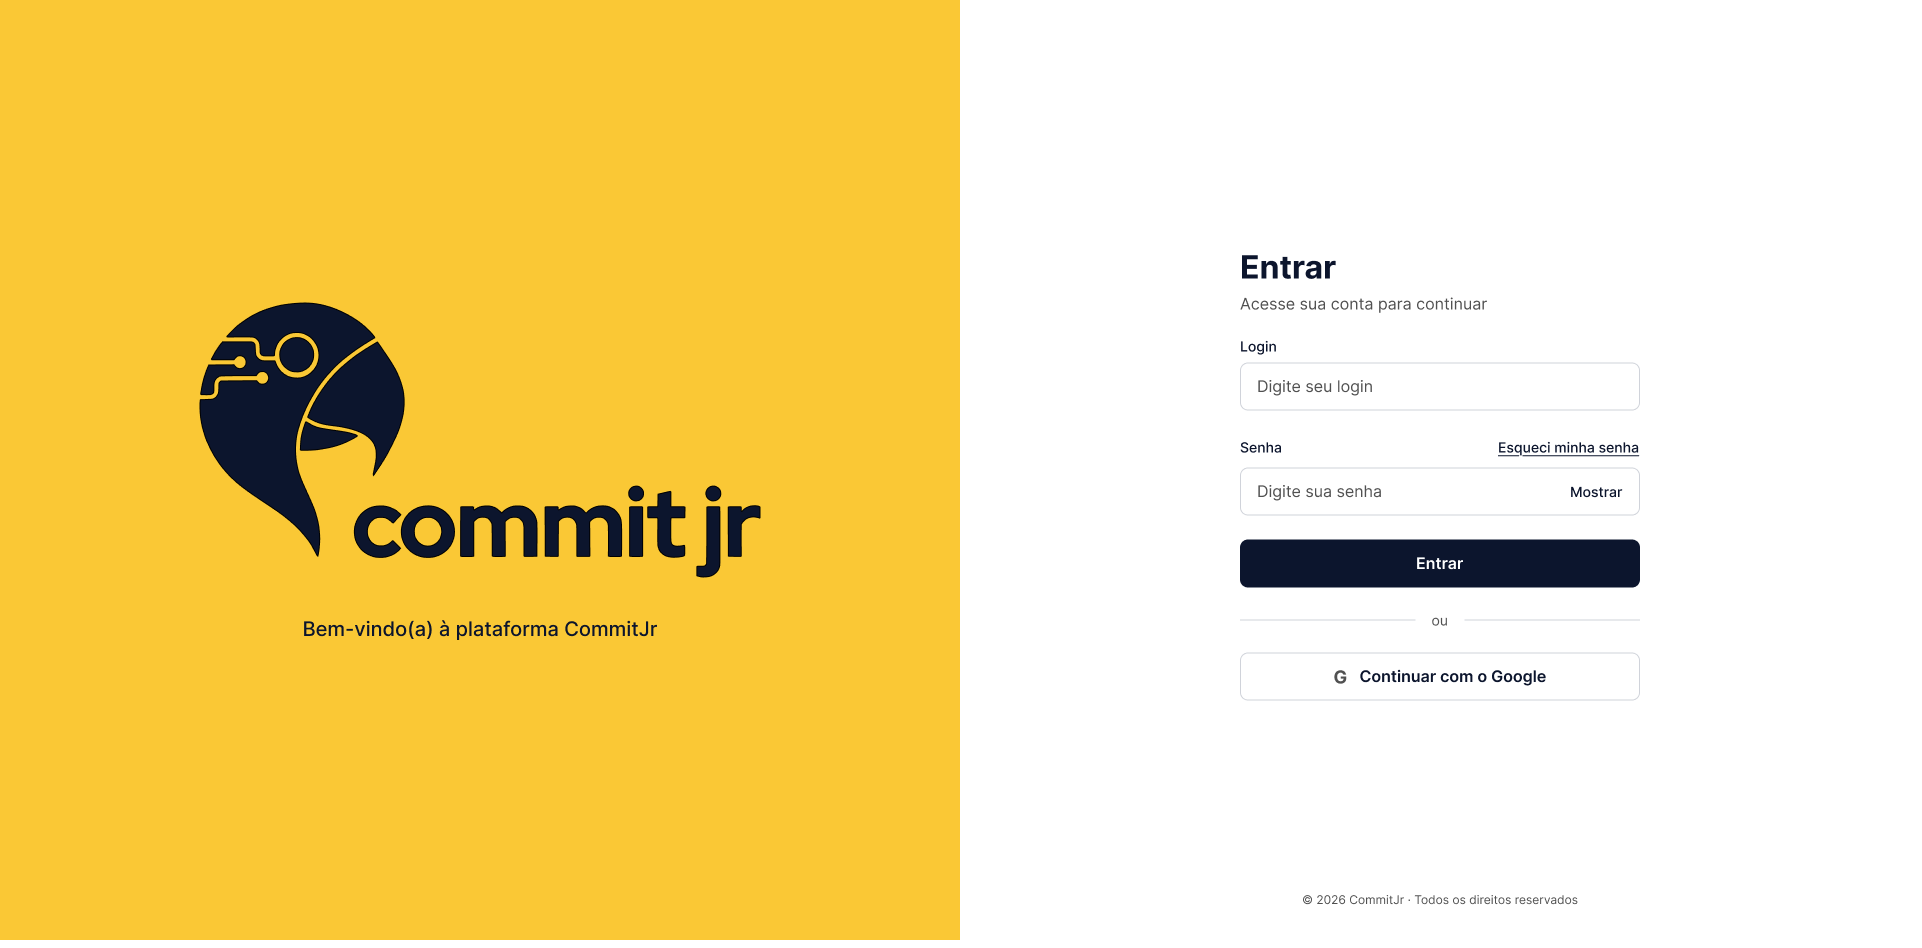
\includegraphics[width=0.88\textwidth]{Telas/login}} \\
\hline
\end{tabular}
\end{center}

\begin{center}
\begin{tabular}{|p{2.0cm}|p{11.5cm}|}
\hline
\textbf{PT-002} & \textbf{Painel Inicial (destino após o login) (UC-01)} \\
\hline
\multicolumn{2}{|c|}{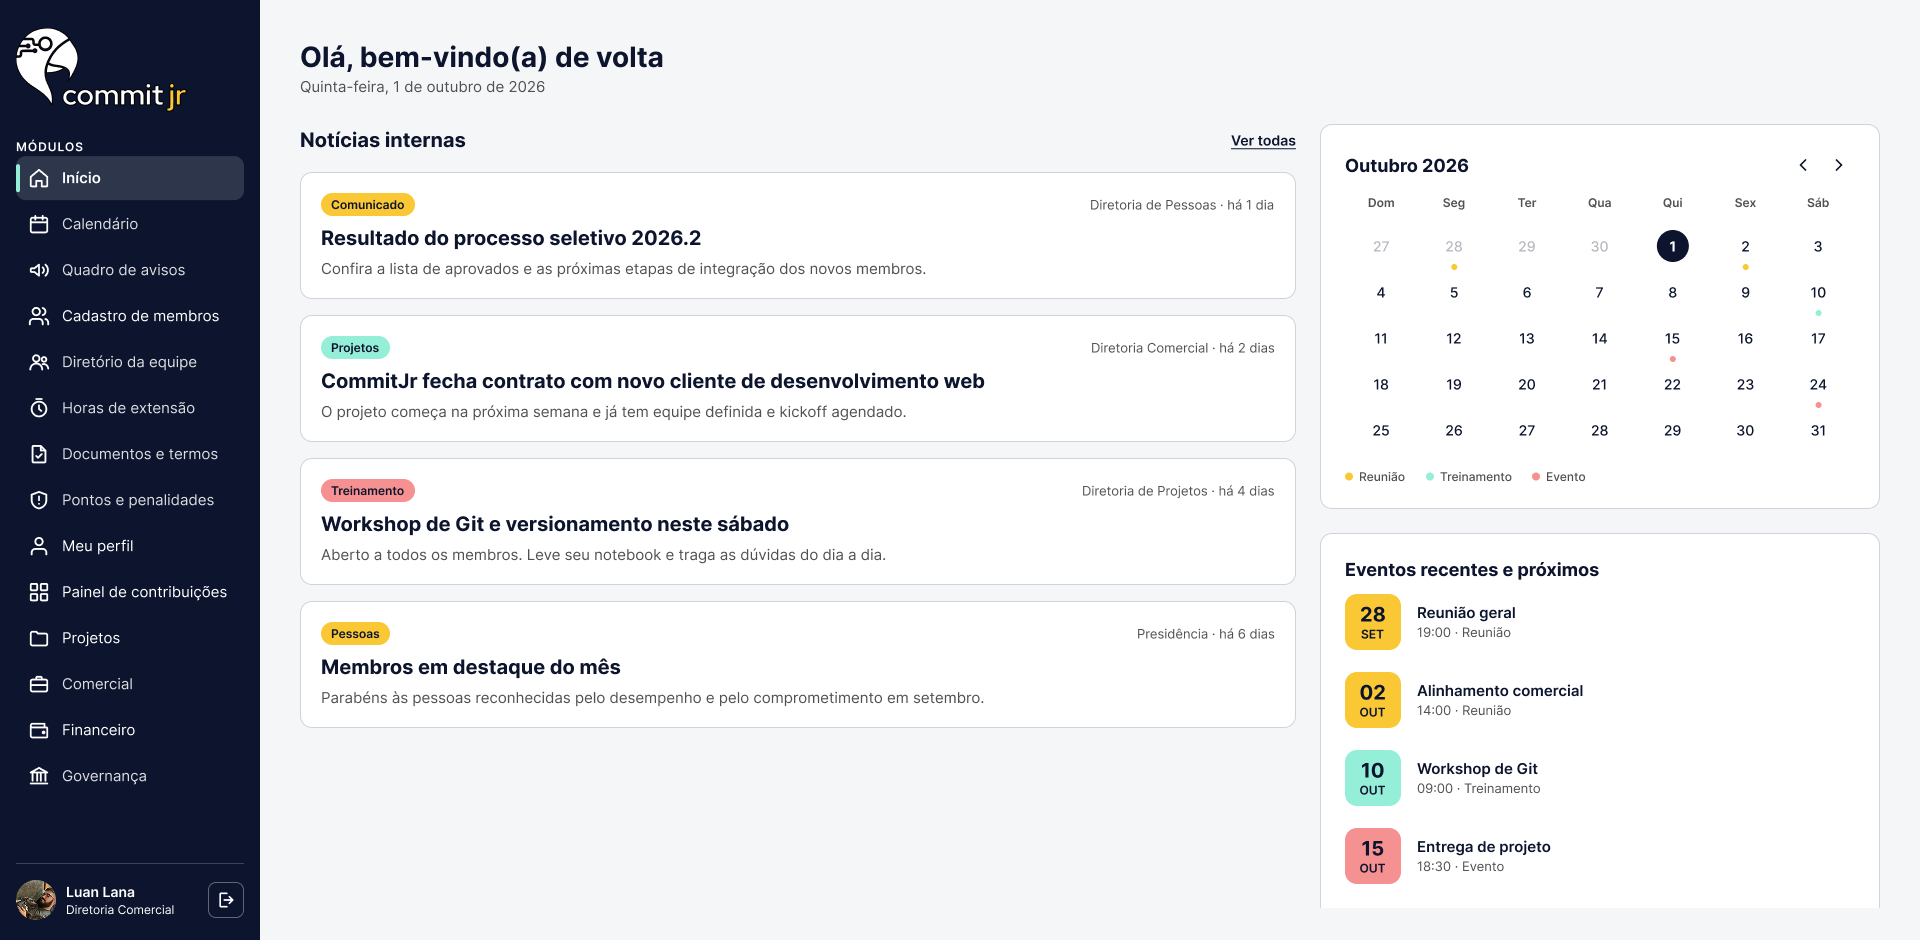
\includegraphics[width=0.88\textwidth]{Telas/inicio}} \\
\hline
\end{tabular}
\end{center}

\begin{center}
\begin{tabular}{|p{2.0cm}|p{11.5cm}|}
\hline
\textbf{PT-003} & \textbf{Meu Perfil de Membro (UC-02)} \\
\hline
\multicolumn{2}{|c|}{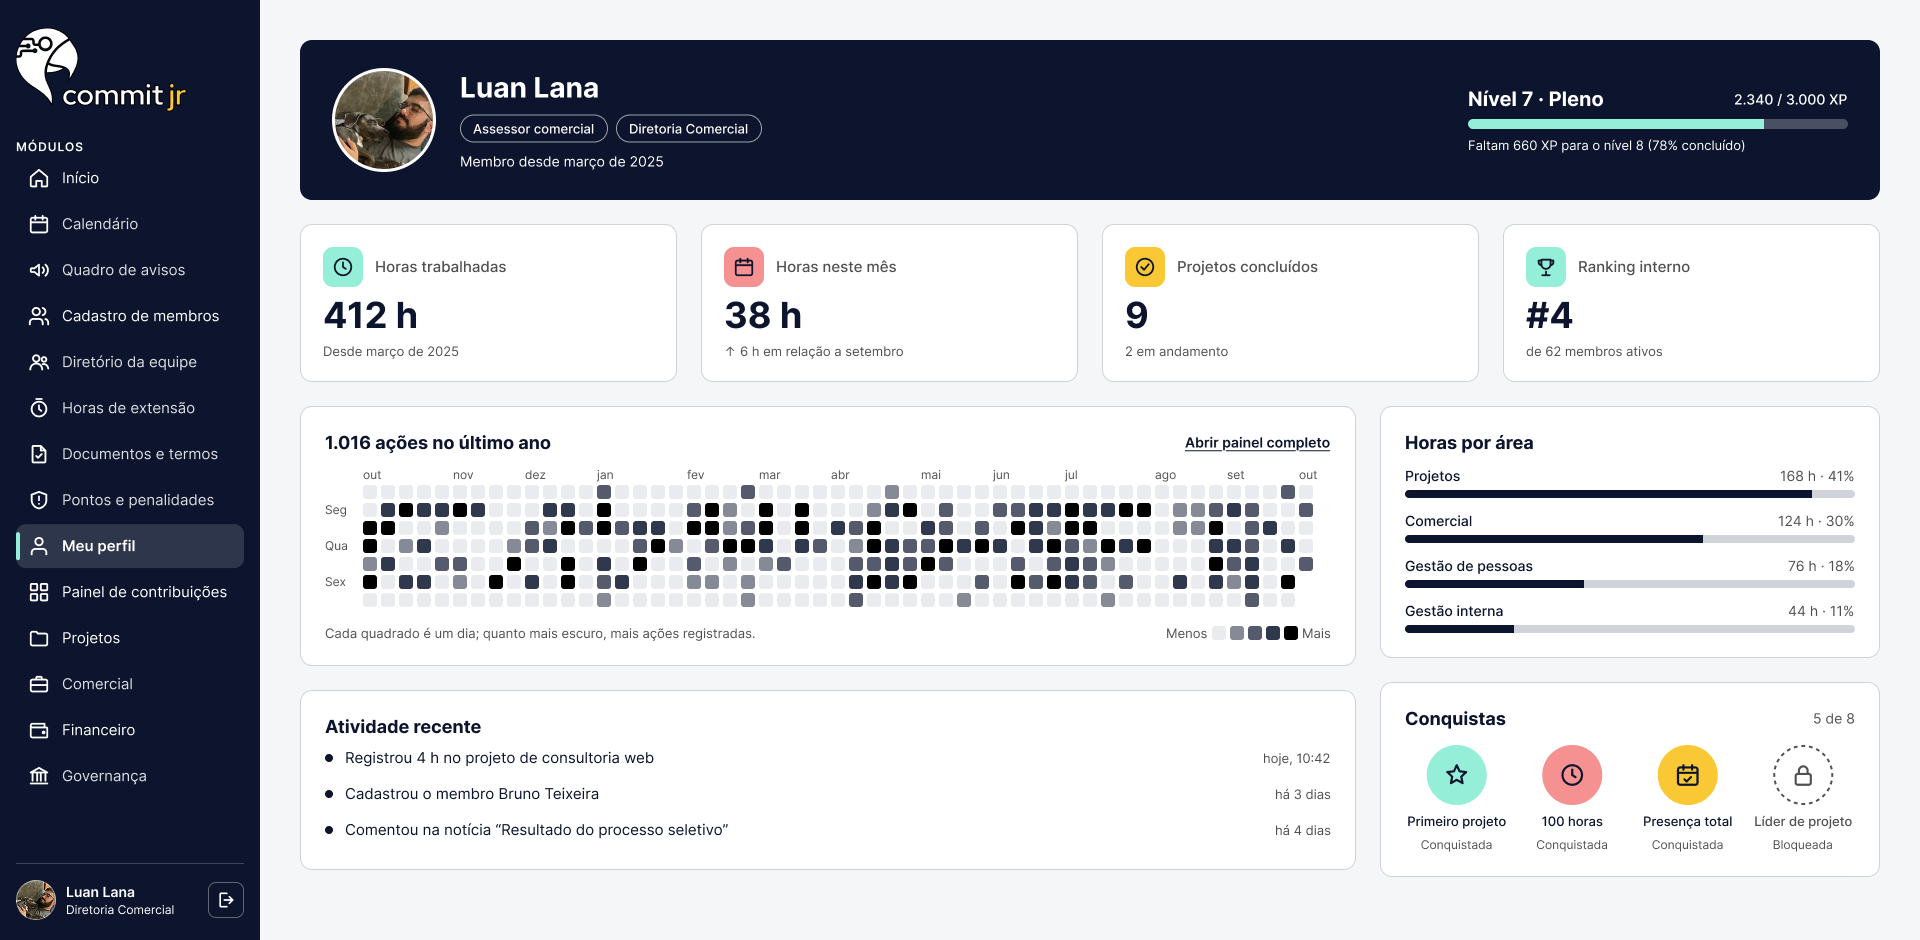
\includegraphics[width=0.88\textwidth]{Telas/meu-perfil}} \\
\hline
\end{tabular}
\end{center}

\begin{center}
\begin{tabular}{|p{2.0cm}|p{11.5cm}|}
\hline
\textbf{PT-004} & \textbf{Cadastro de Membros -- Listagem Geral (UC-09)} \\
\hline
\multicolumn{2}{|c|}{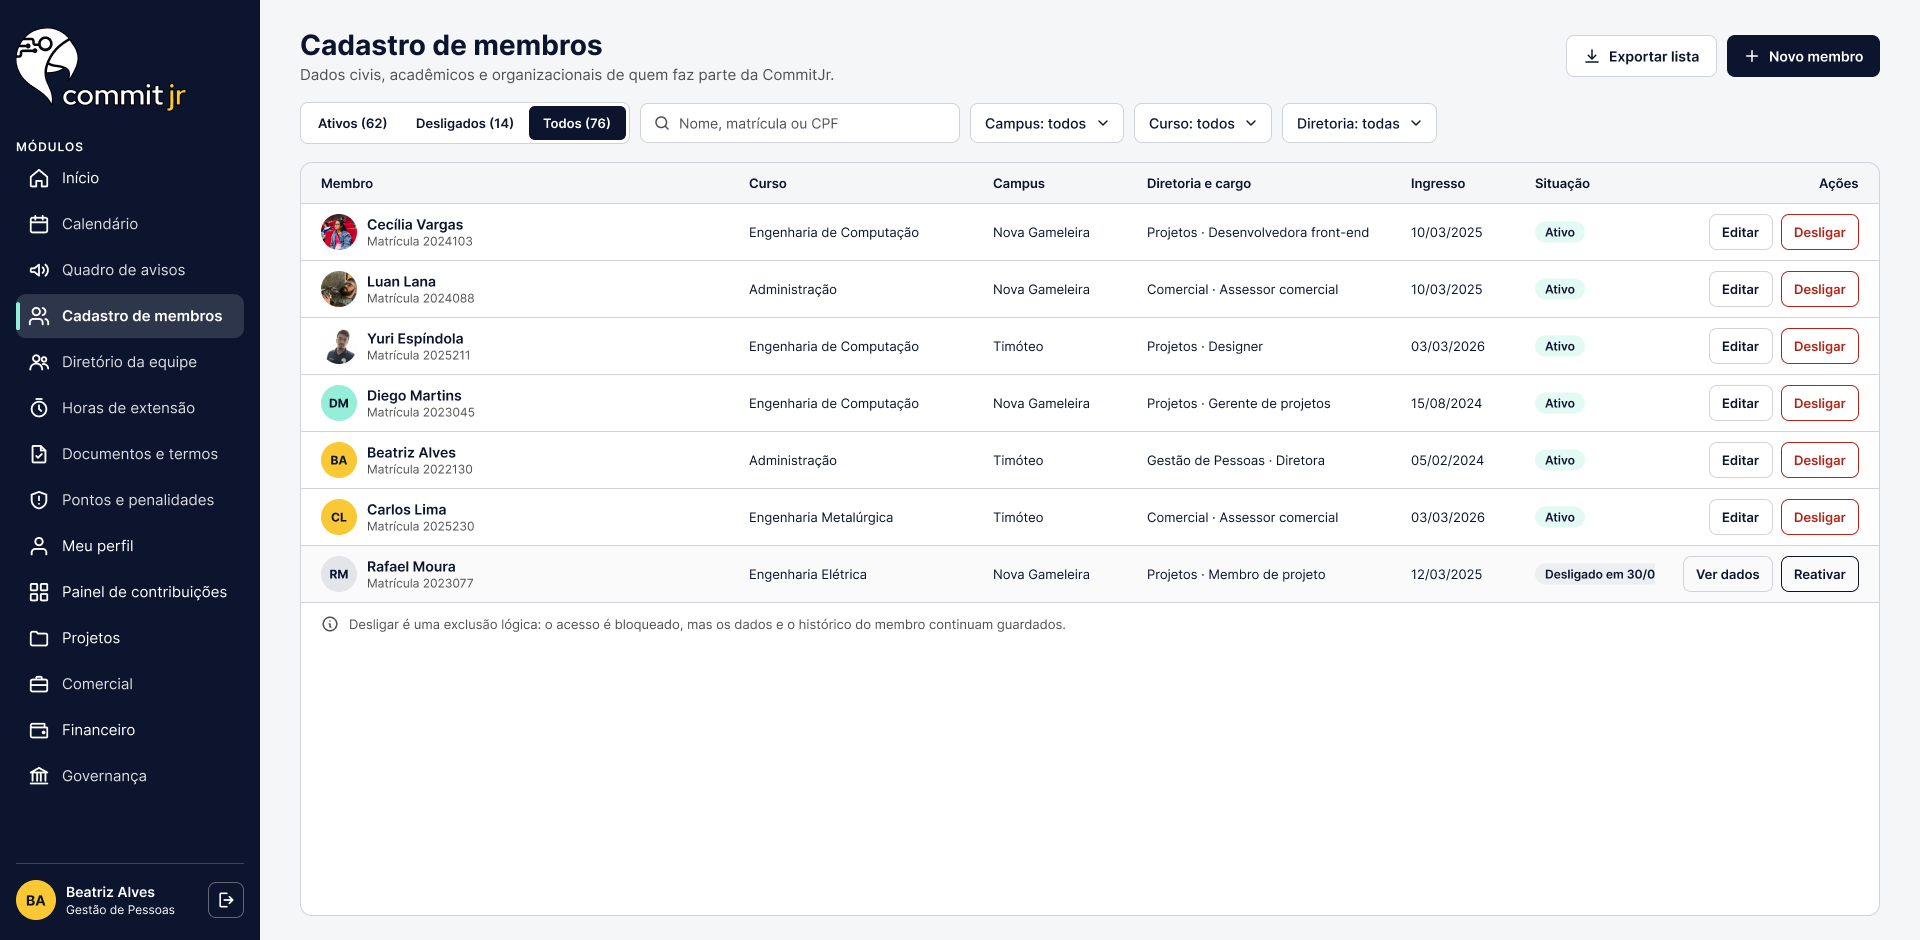
\includegraphics[width=0.88\textwidth]{Telas/membros-lista}} \\
\hline
\end{tabular}
\end{center}

\begin{center}
\begin{tabular}{|p{2.0cm}|p{11.5cm}|}
\hline
\textbf{PT-005} & \textbf{Cadastro de Membros -- Edição de Dados (UC-09)} \\
\hline
\multicolumn{2}{|c|}{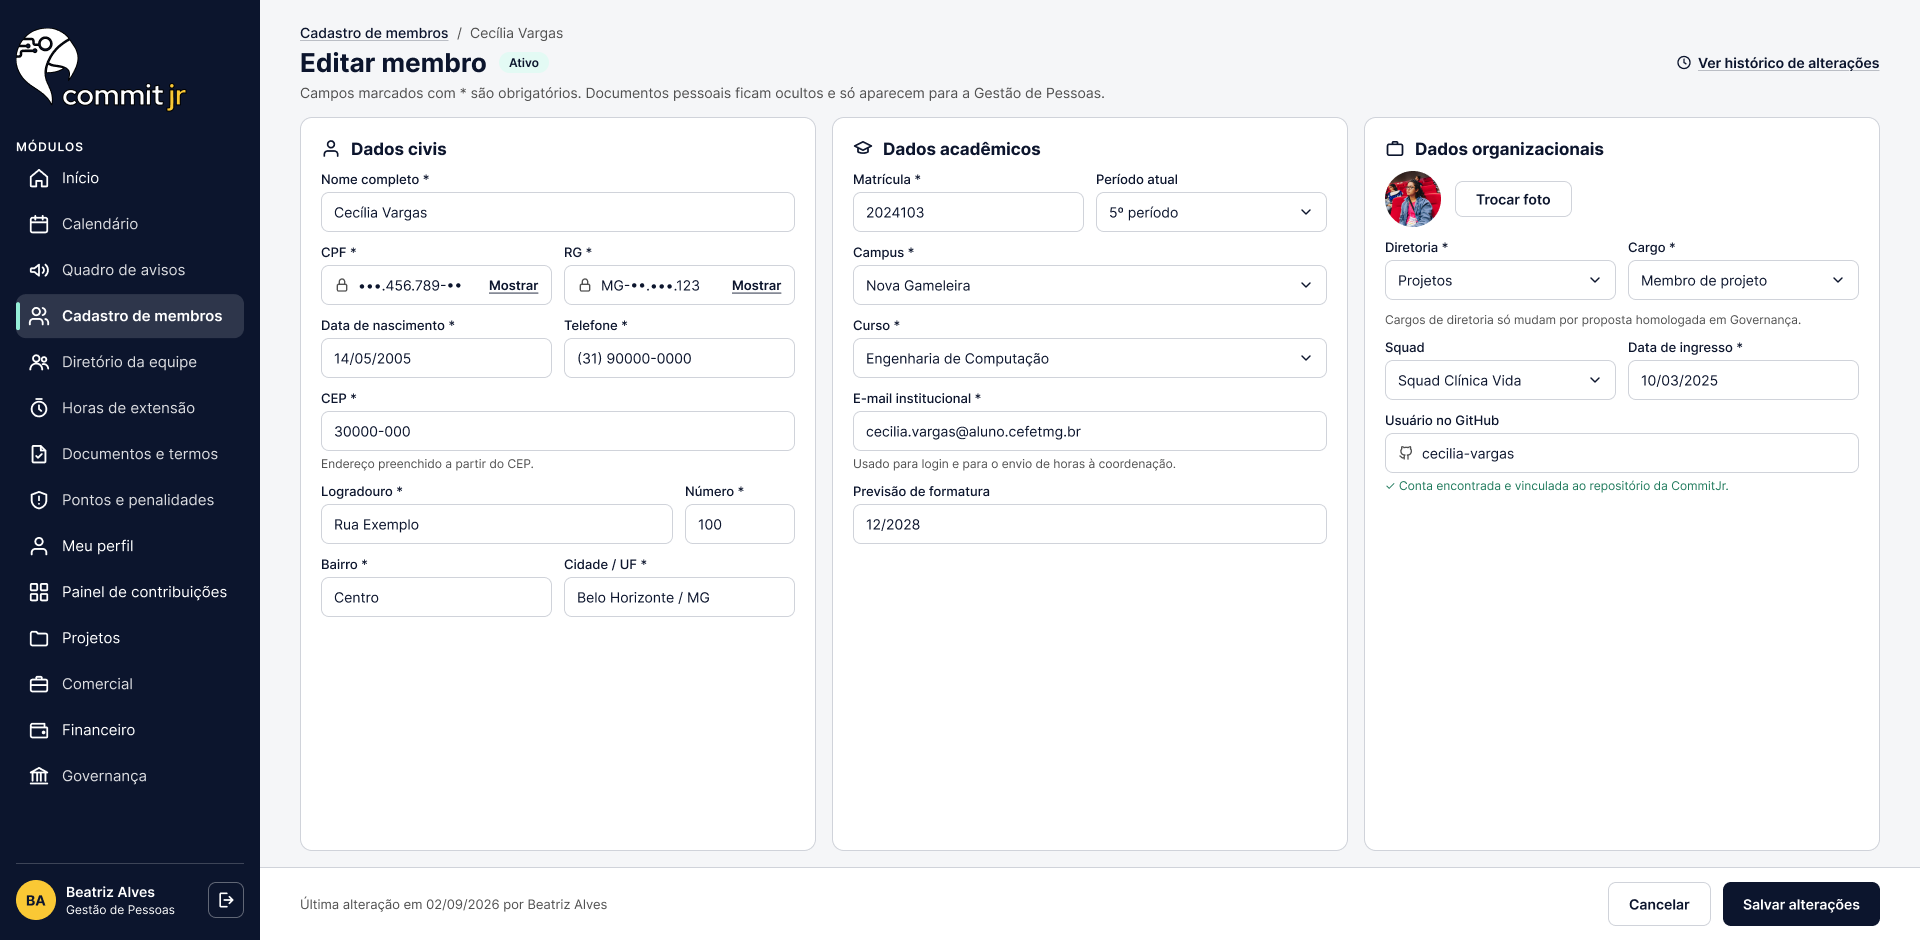
\includegraphics[width=0.88\textwidth]{Telas/membros-editar}} \\
\hline
\end{tabular}
\end{center}

\begin{center}
\begin{tabular}{|p{2.0cm}|p{11.5cm}|}
\hline
\textbf{PT-006} & \textbf{Cadastro de Membros -- Desligamento e Inativação Lógica (UC-09)} \\
\hline
\multicolumn{2}{|c|}{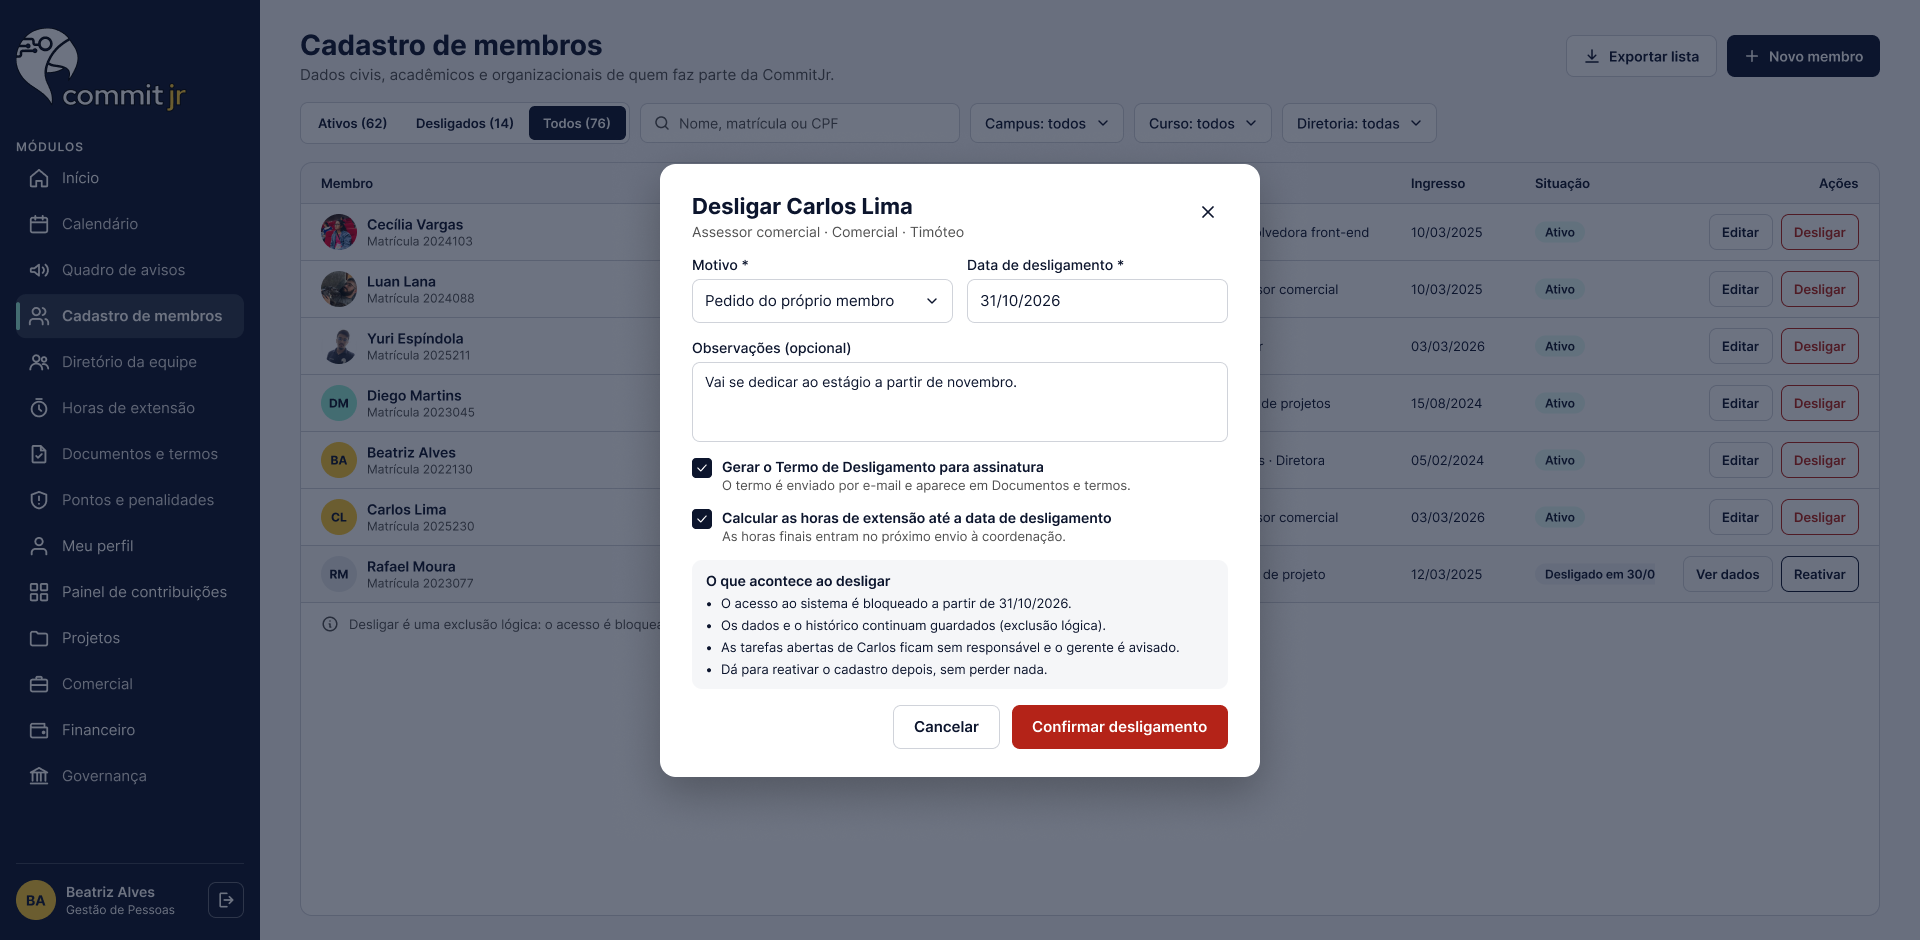
\includegraphics[width=0.88\textwidth]{Telas/membros-desligar}} \\
\hline
\end{tabular}
\end{center}

\begin{center}
\begin{tabular}{|p{2.0cm}|p{11.5cm}|}
\hline
\textbf{PT-007} & \textbf{Diretório Corporativo da Equipe (UC-03)} \\
\hline
\multicolumn{2}{|c|}{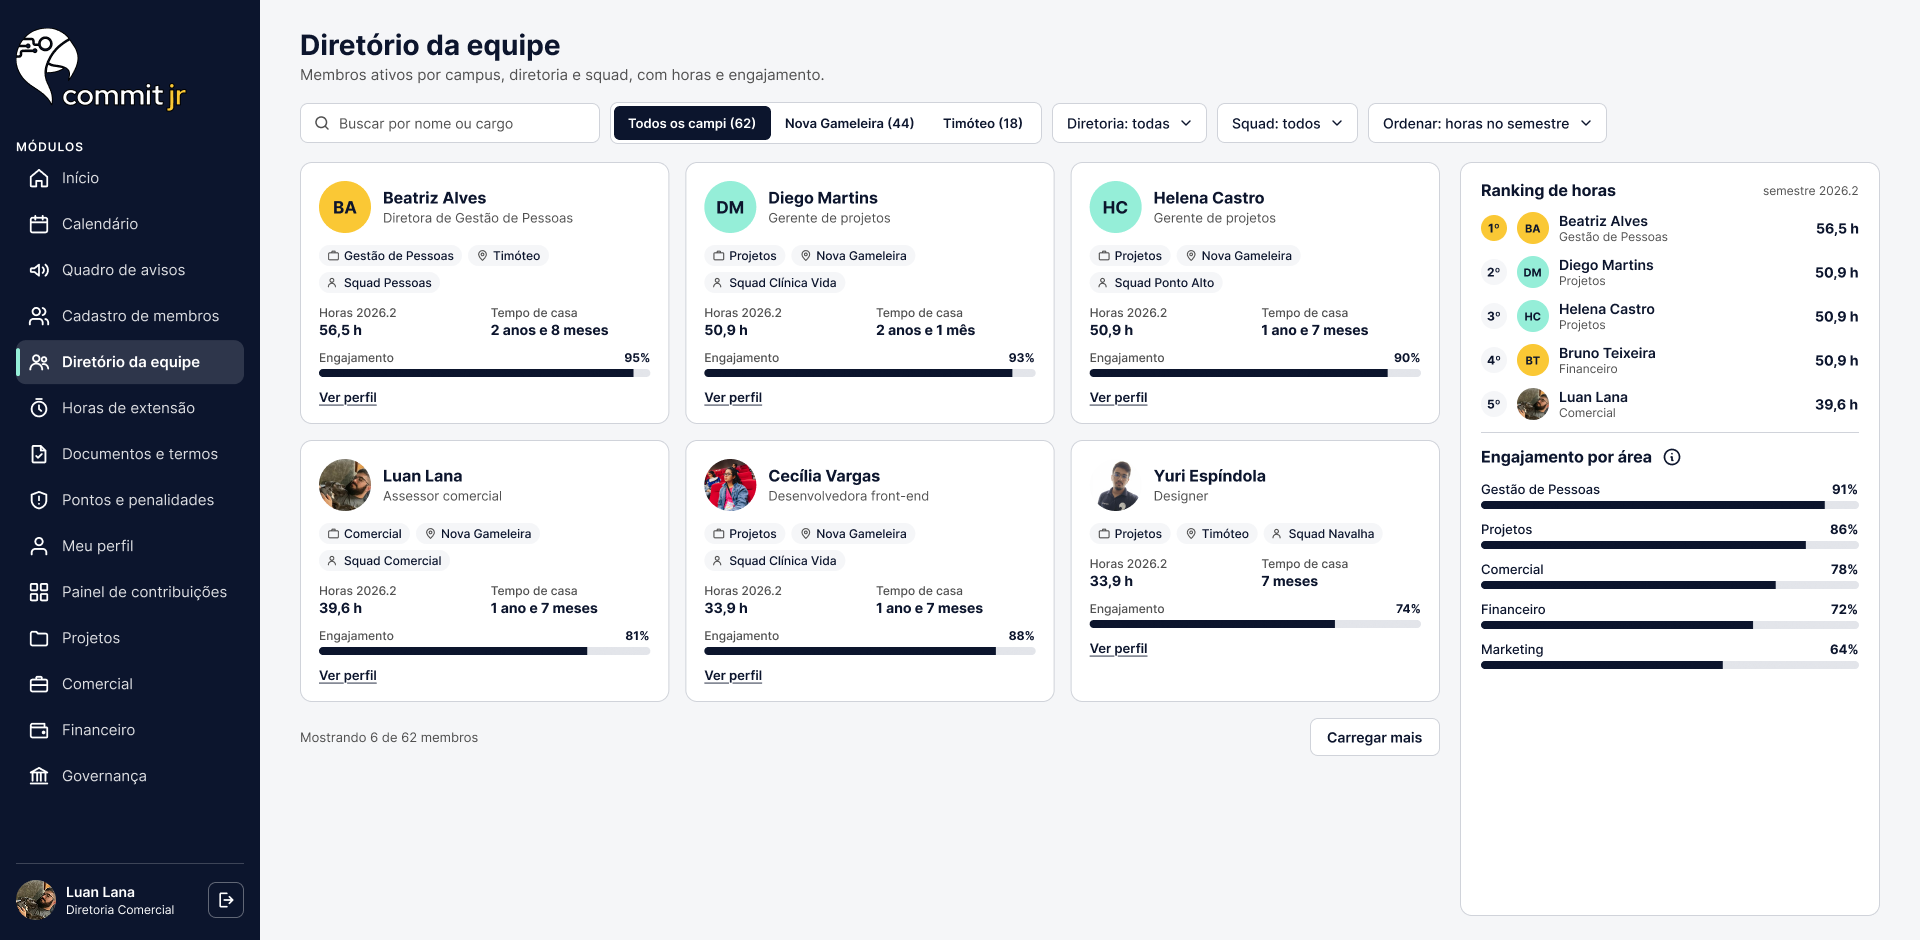
\includegraphics[width=0.88\textwidth]{Telas/diretorio-equipe}} \\
\hline
\end{tabular}
\end{center}

\begin{center}
\begin{tabular}{|p{2.0cm}|p{11.5cm}|}
\hline
\textbf{PT-008} & \textbf{Documentos e Termos Jurídicos (UC-08)} \\
\hline
\multicolumn{2}{|c|}{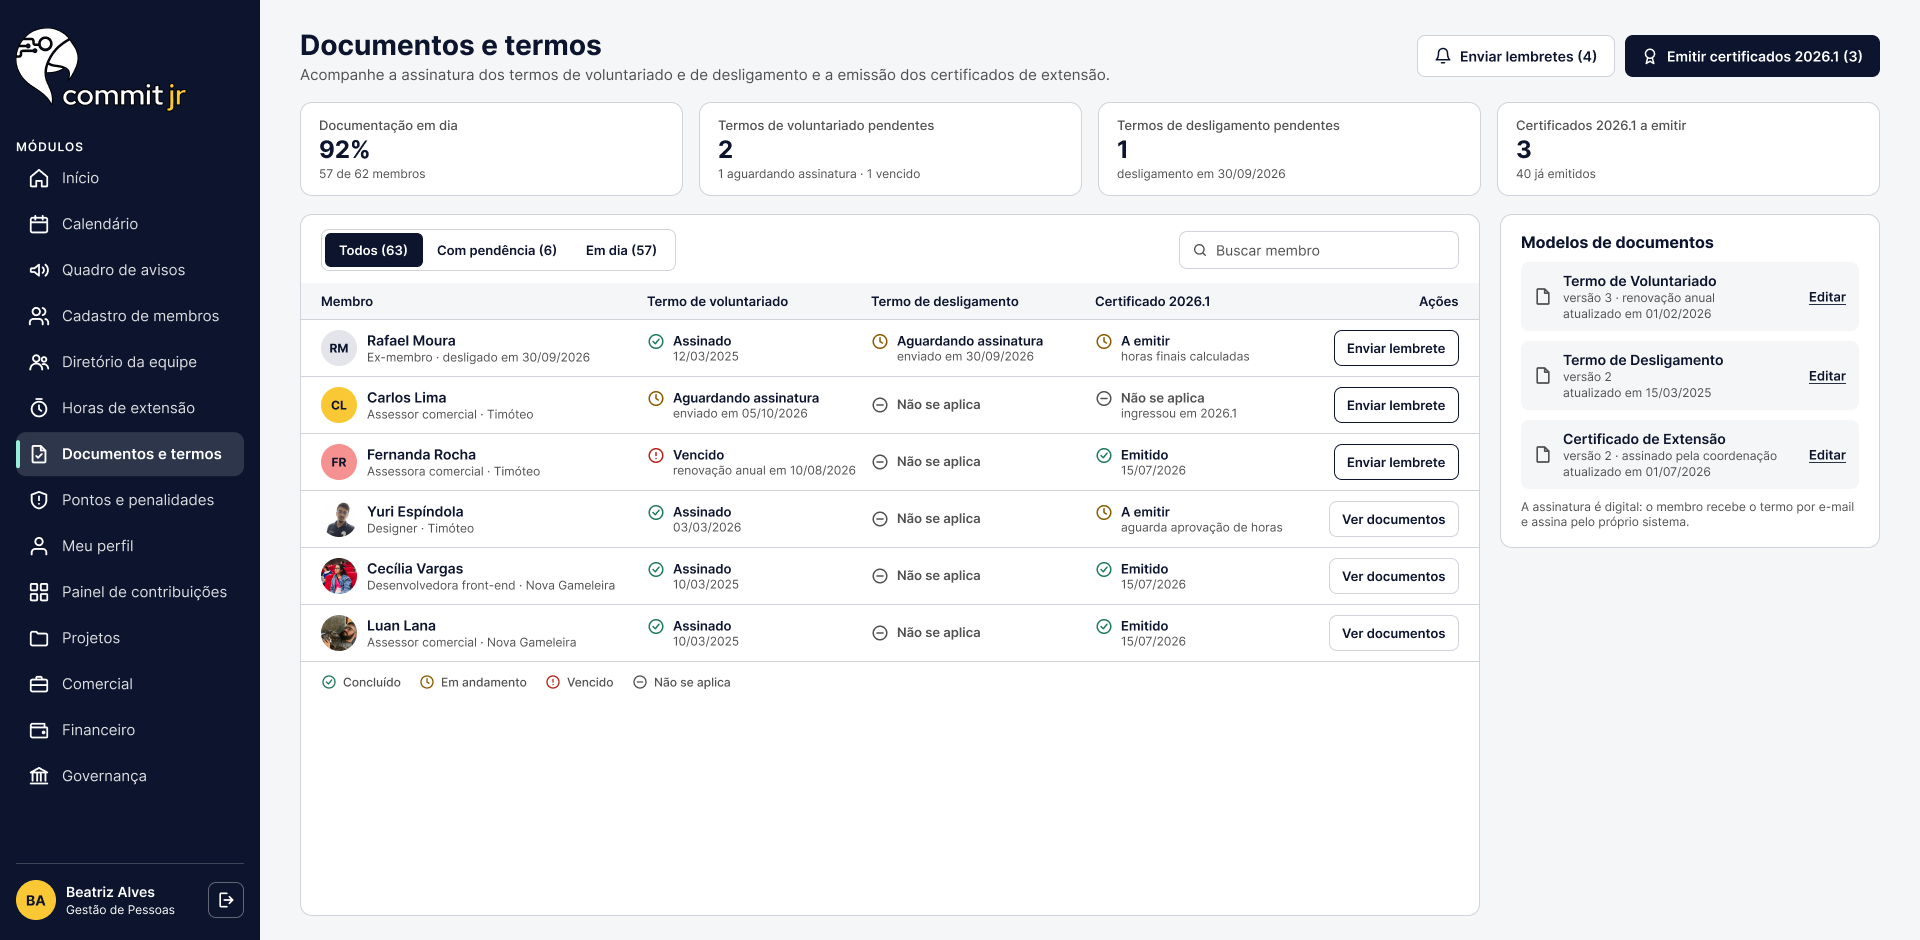
\includegraphics[width=0.88\textwidth]{Telas/documentos-e-termos}} \\
\hline
\end{tabular}
\end{center}

\begin{center}
\begin{tabular}{|p{2.0cm}|p{11.5cm}|}
\hline
\textbf{PT-009} & \textbf{Horas de Extensão -- Regras por Cargo (UC-12)} \\
\hline
\multicolumn{2}{|c|}{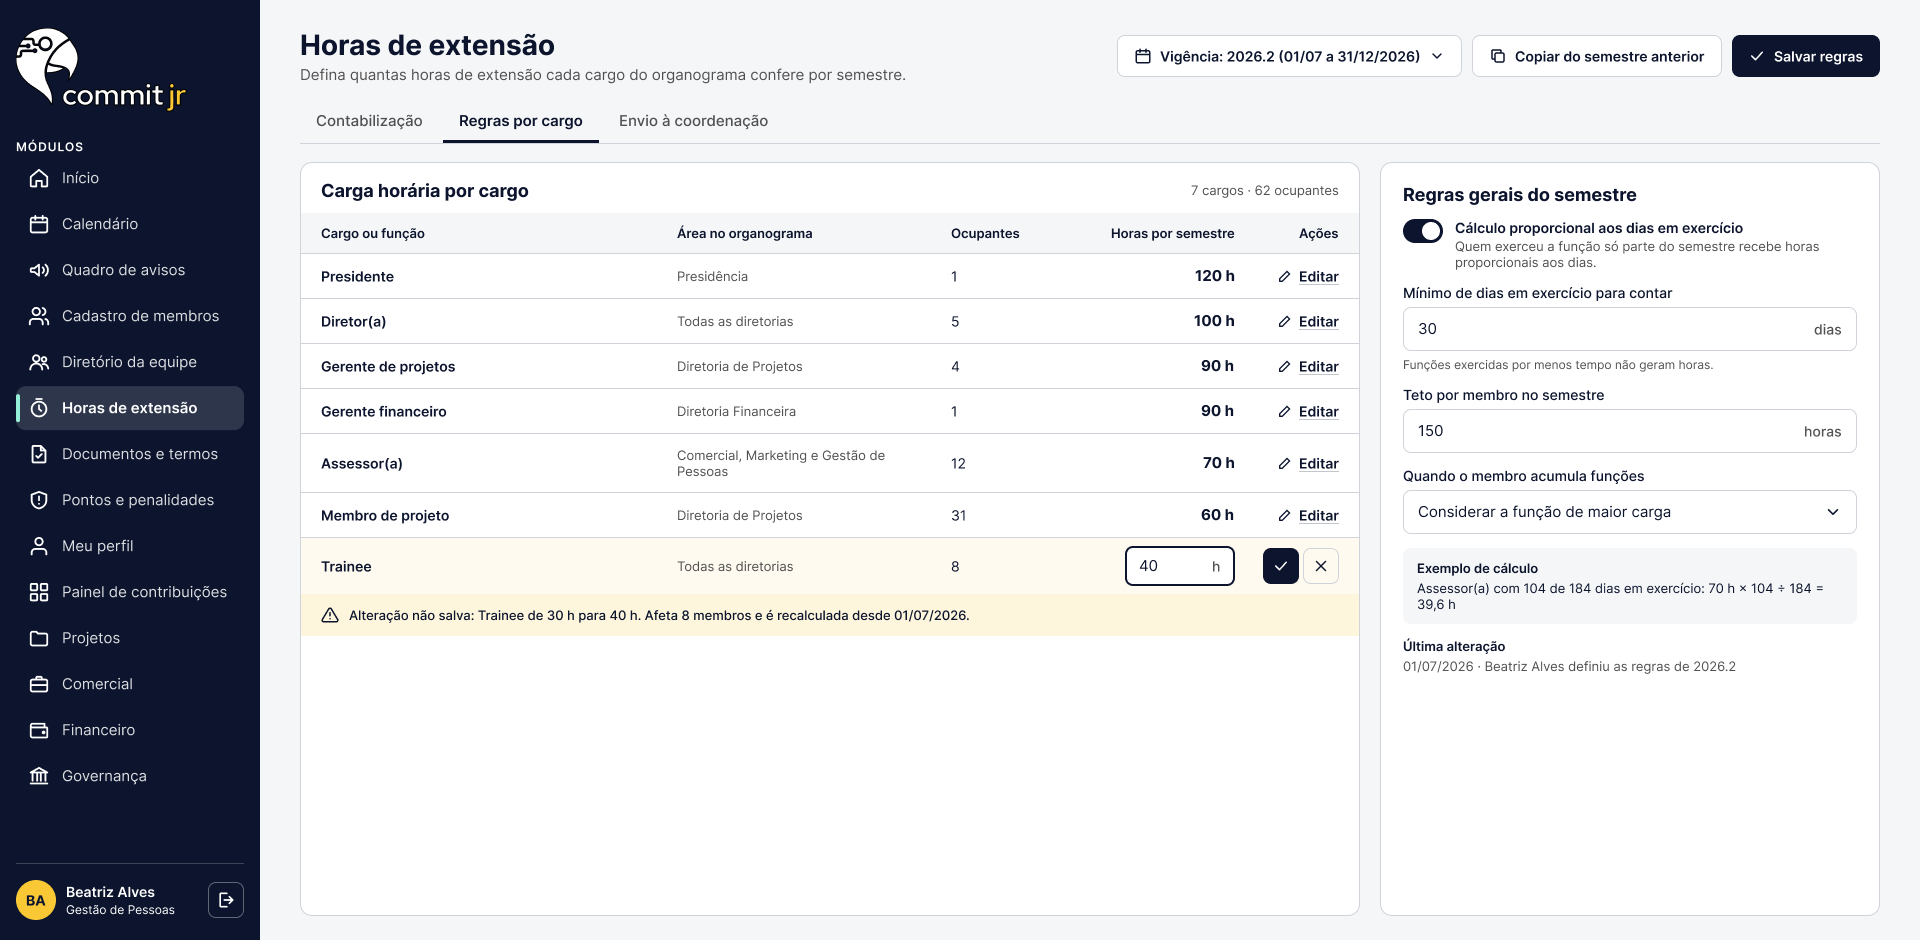
\includegraphics[width=0.88\textwidth]{Telas/horas-regras-por-cargo}} \\
\hline
\end{tabular}
\end{center}

\begin{center}
\begin{tabular}{|p{2.0cm}|p{11.5cm}|}
\hline
\textbf{PT-010} & \textbf{Horas de Extensão -- Contabilização Automática (UC-13)} \\
\hline
\multicolumn{2}{|c|}{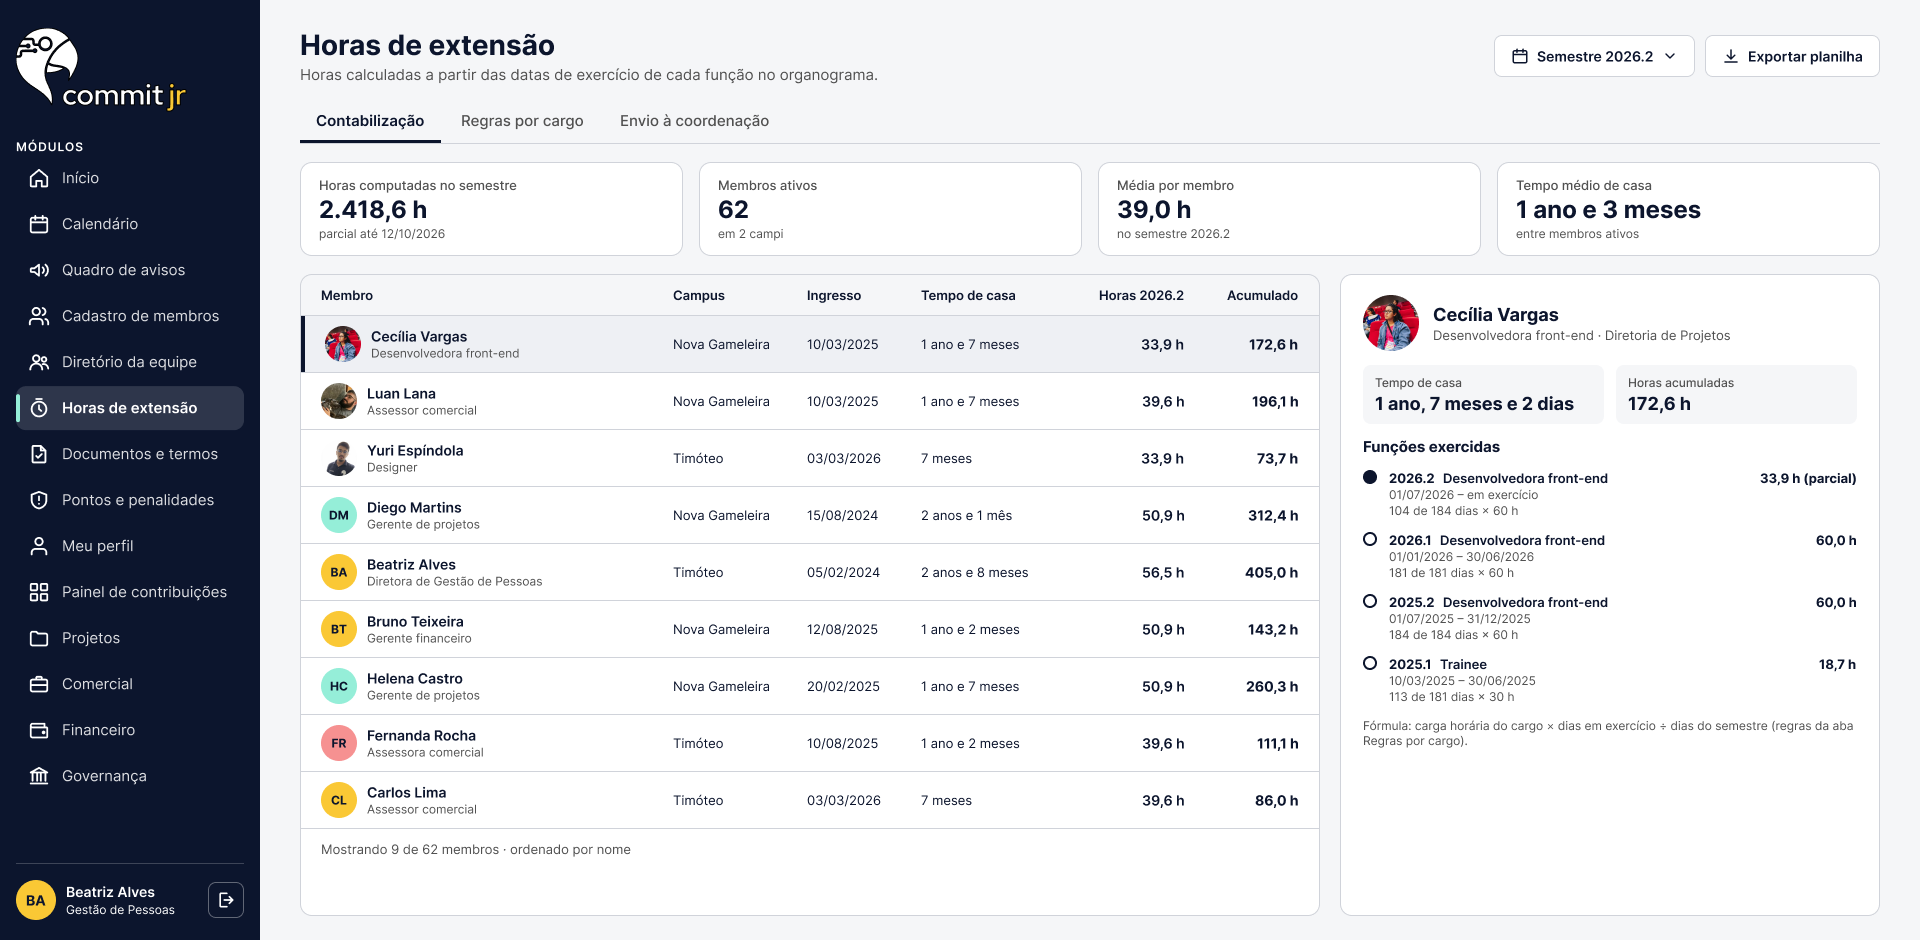
\includegraphics[width=0.88\textwidth]{Telas/horas-contabilizacao}} \\
\hline
\end{tabular}
\end{center}

\begin{center}
\begin{tabular}{|p{2.0cm}|p{11.5cm}|}
\hline
\textbf{PT-011} & \textbf{Horas de Extensão -- Envio ao Professor Orientador (UC-14)} \\
\hline
\multicolumn{2}{|c|}{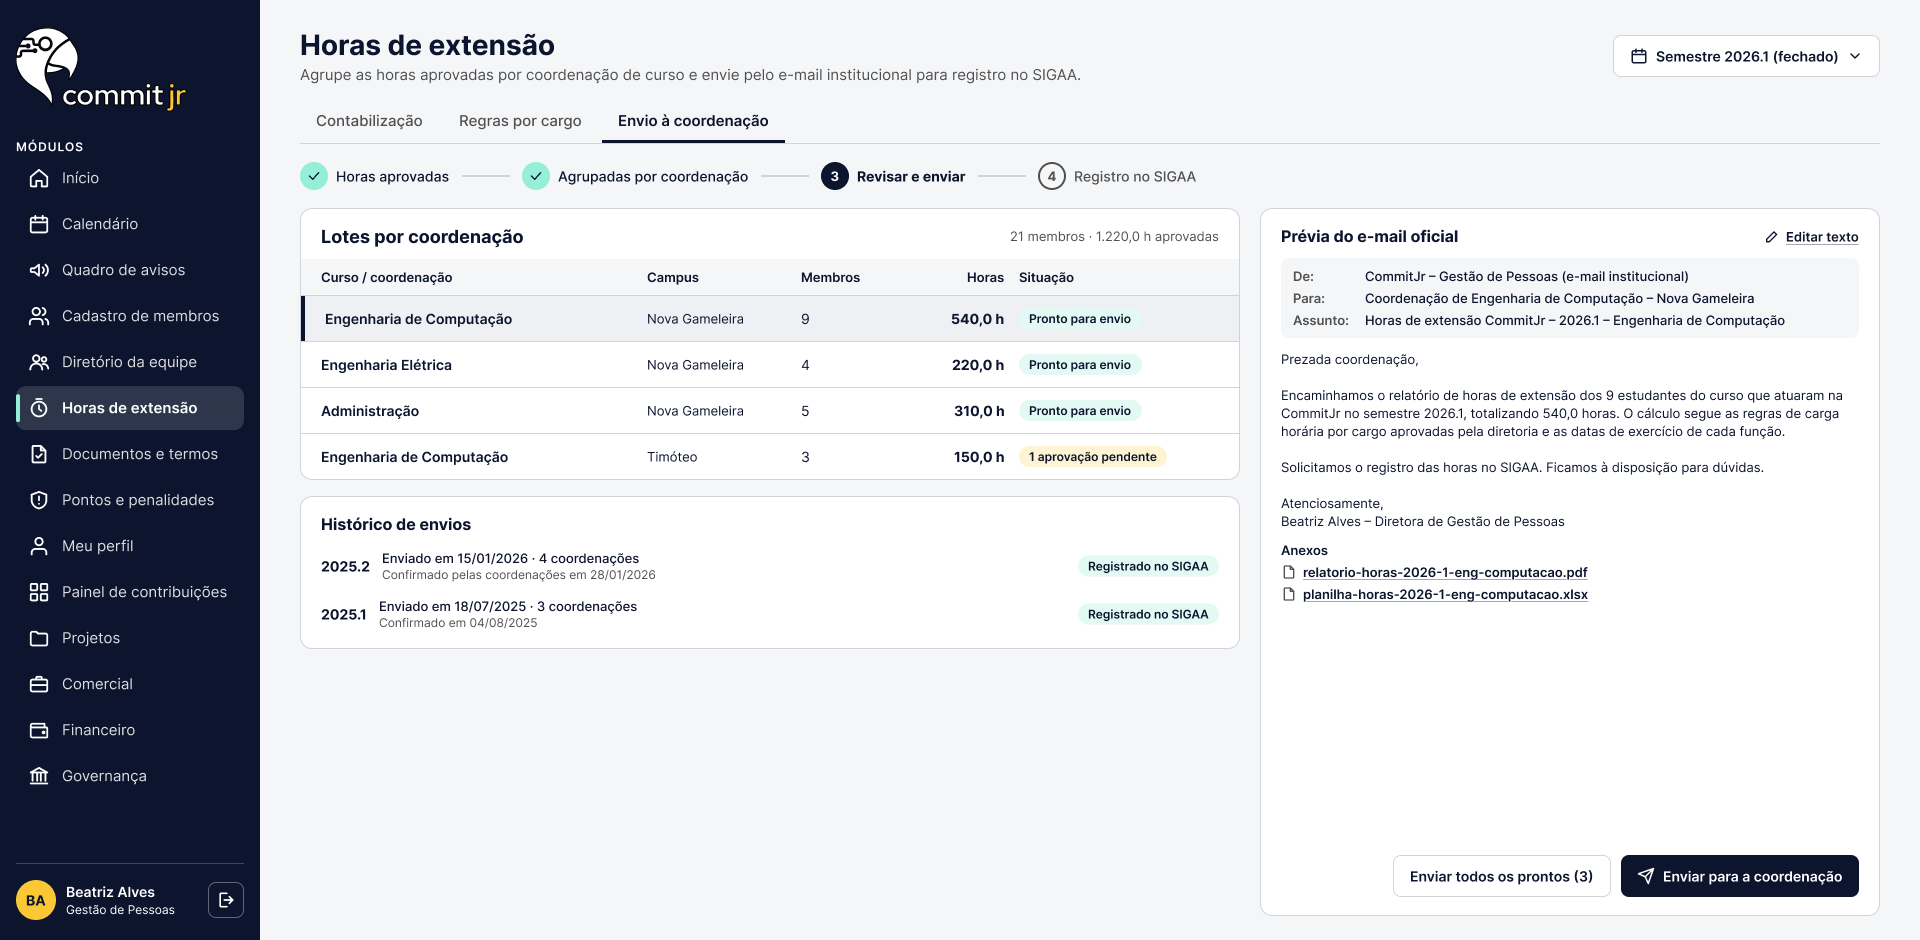
\includegraphics[width=0.88\textwidth]{Telas/horas-envio-coordenacao}} \\
\hline
\end{tabular}
\end{center}

\begin{center}
\begin{tabular}{|p{2.0cm}|p{11.5cm}|}
\hline
\textbf{PT-012} & \textbf{Pontos e Penalidades -- Listagem de Membros (UC-15)} \\
\hline
\multicolumn{2}{|c|}{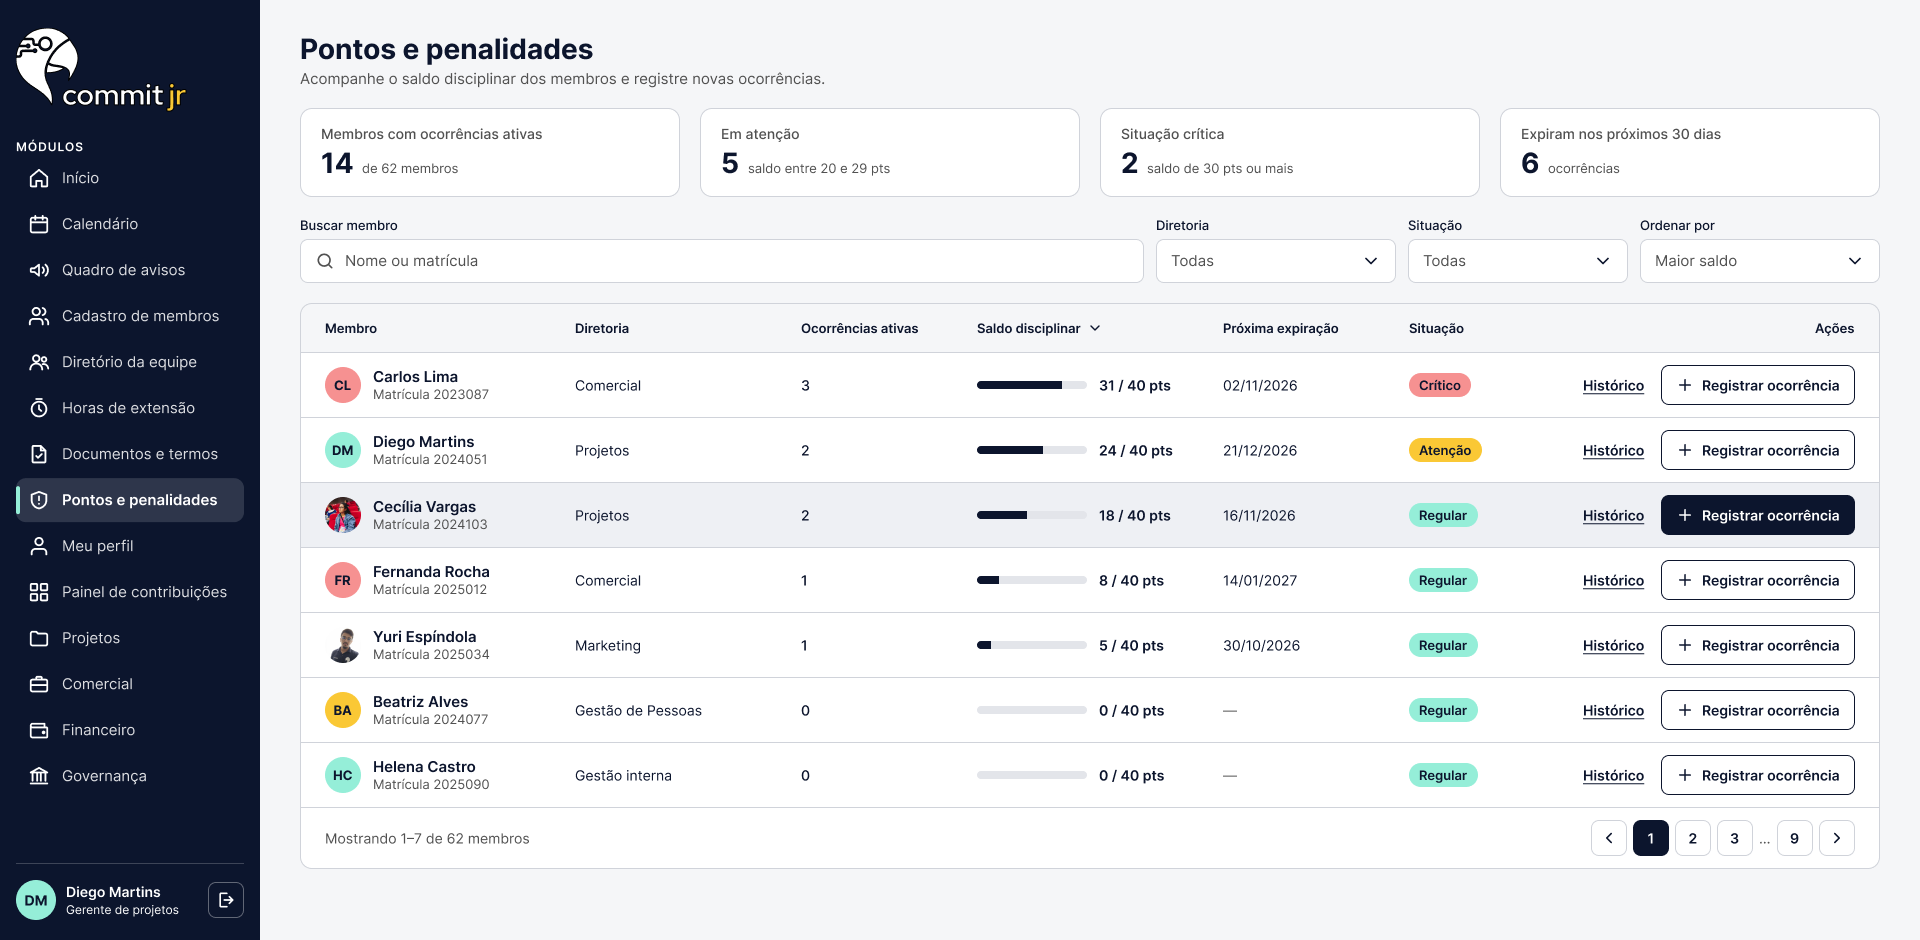
\includegraphics[width=0.88\textwidth]{Telas/pontos-lista-membros}} \\
\hline
\end{tabular}
\end{center}

\begin{center}
\begin{tabular}{|p{2.0cm}|p{11.5cm}|}
\hline
\textbf{PT-013} & \textbf{Pontos e Penalidades -- Registro de Ocorrência (UC-15)} \\
\hline
\multicolumn{2}{|c|}{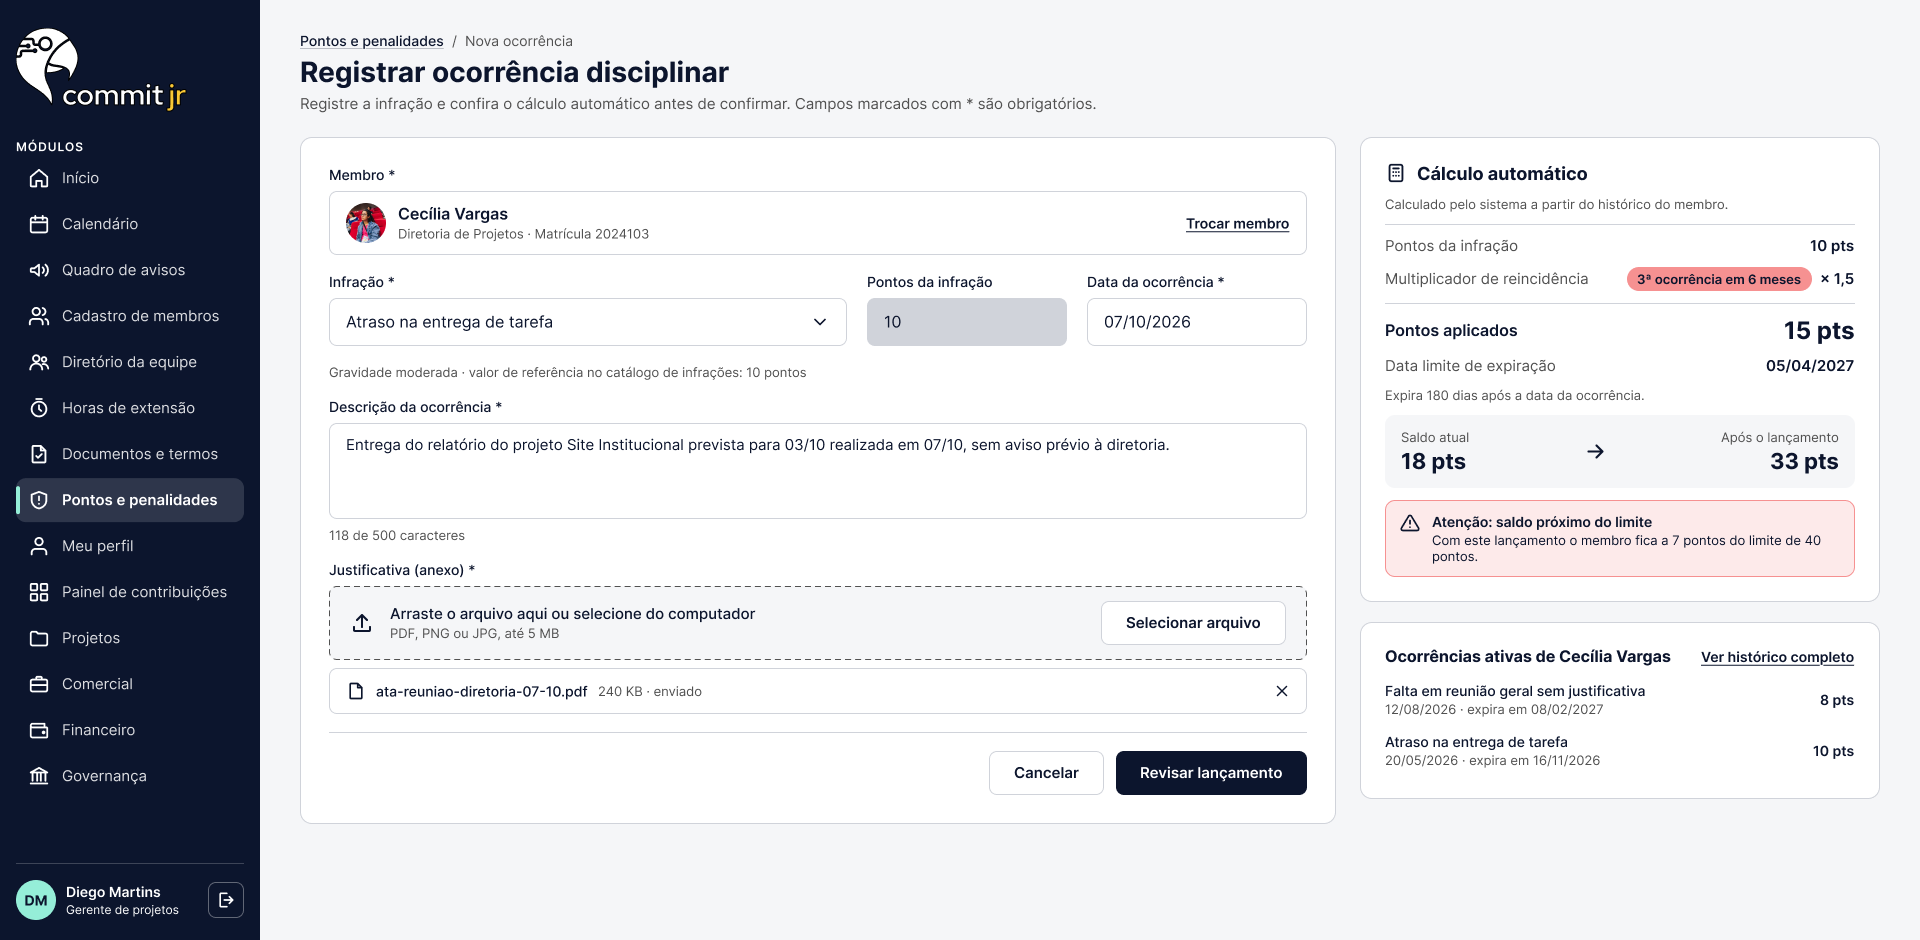
\includegraphics[width=0.88\textwidth]{Telas/pontos-registrar-ocorrencia}} \\
\hline
\end{tabular}
\end{center}

\begin{center}
\begin{tabular}{|p{2.0cm}|p{11.5cm}|}
\hline
\textbf{PT-014} & \textbf{Pontos e Penalidades -- Confirmação de Lançamento (UC-15)} \\
\hline
\multicolumn{2}{|c|}{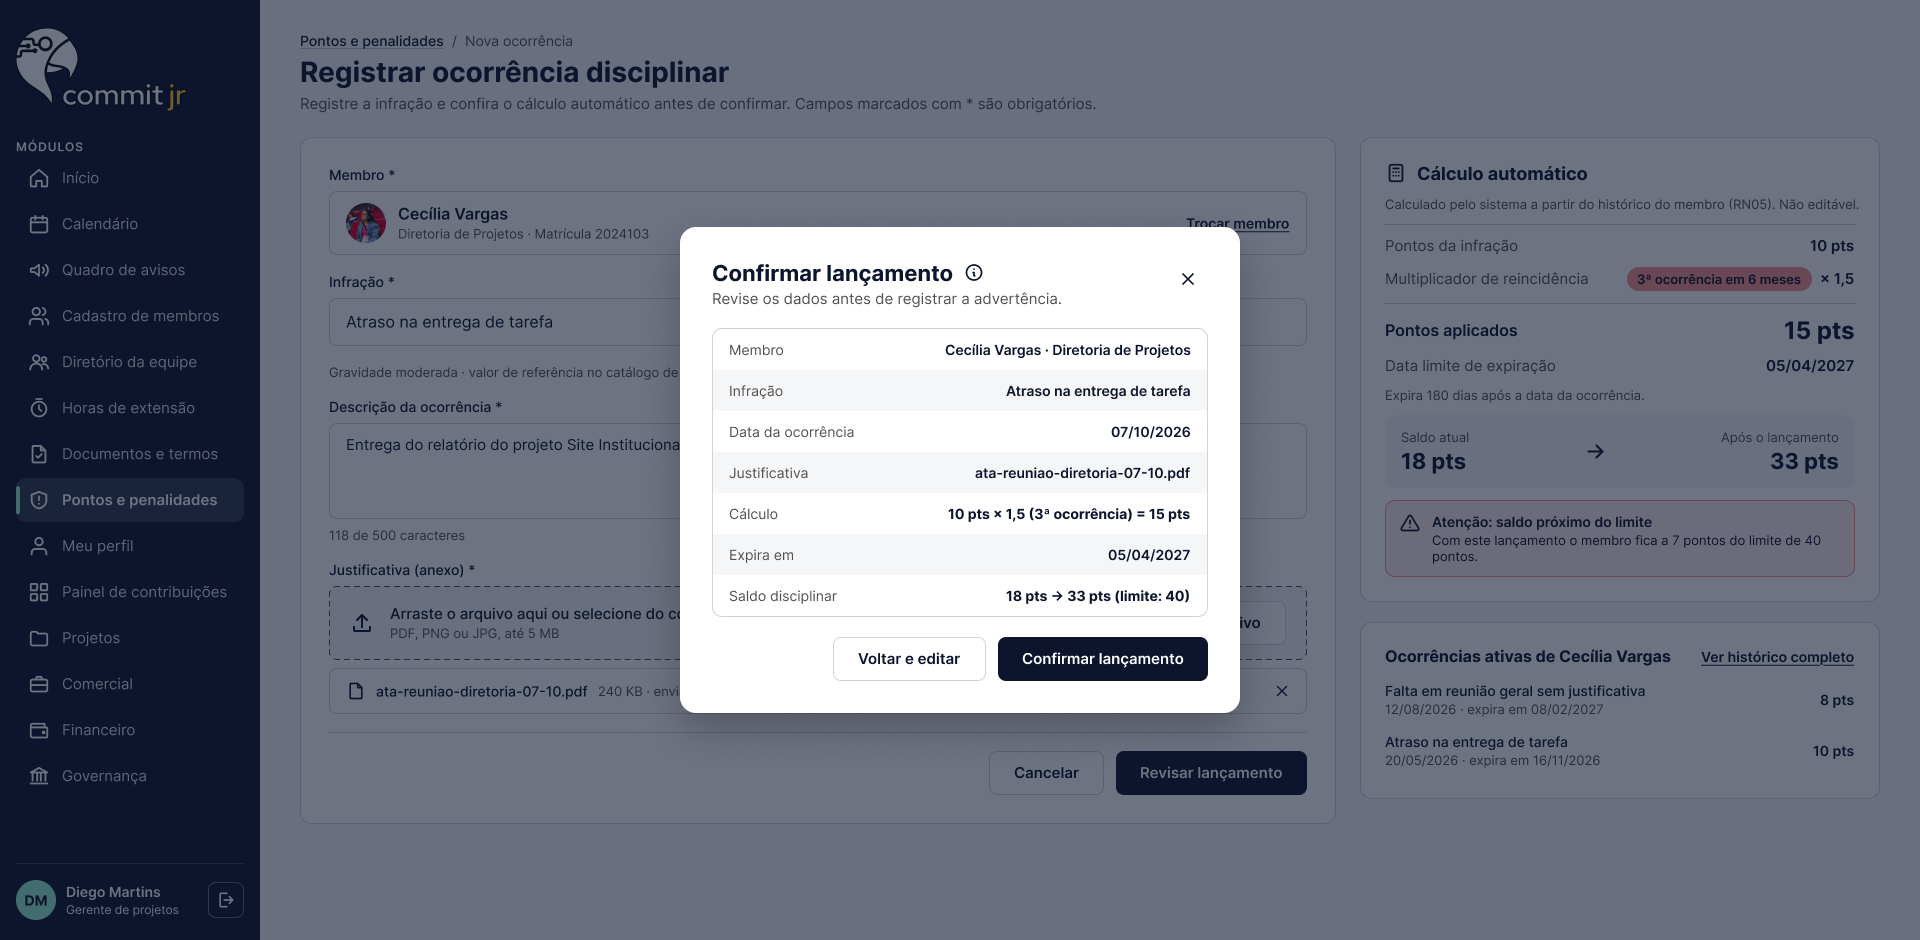
\includegraphics[width=0.88\textwidth]{Telas/pontos-confirmar-lancamento}} \\
\hline
\end{tabular}
\end{center}

\begin{center}
\begin{tabular}{|p{2.0cm}|p{11.5cm}|}
\hline
\textbf{PT-015} & \textbf{Pontos e Penalidades -- Julgar Contestações (UC-11)} \\
\hline
\multicolumn{2}{|c|}{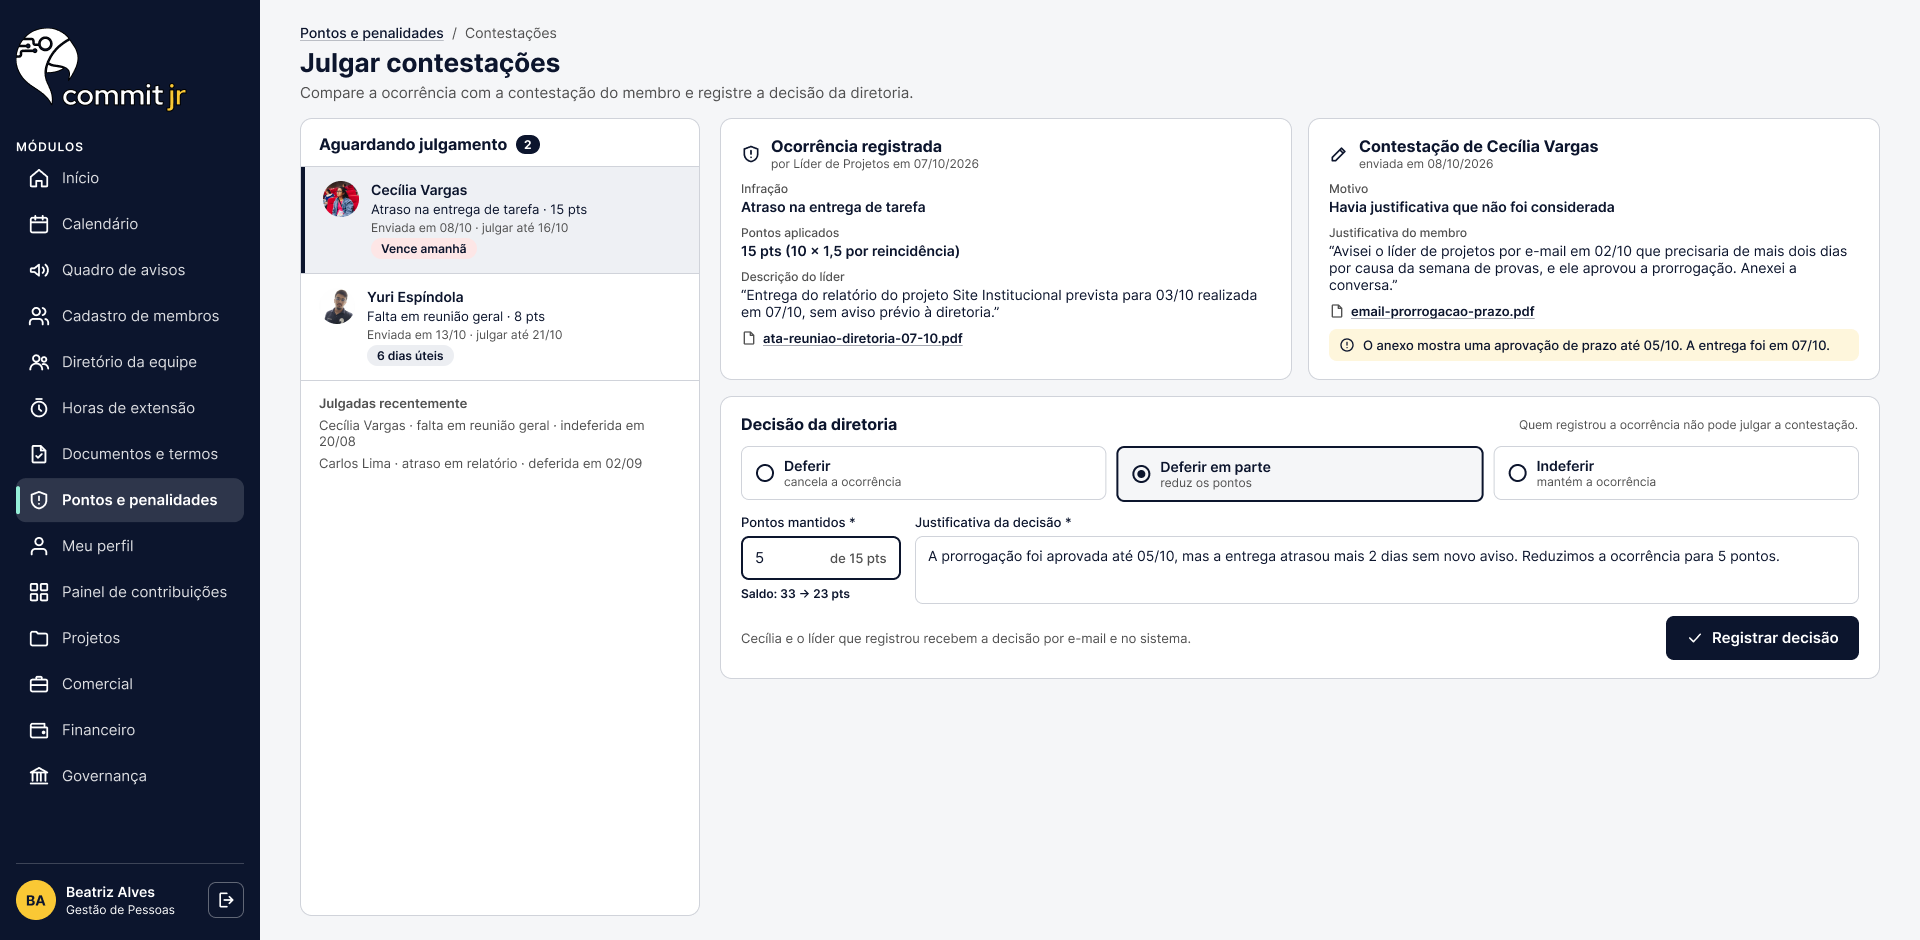
\includegraphics[width=0.88\textwidth]{Telas/pontos-julgar-contestacoes}} \\
\hline
\end{tabular}
\end{center}

\begin{center}
\begin{tabular}{|p{2.0cm}|p{11.5cm}|}
\hline
\textbf{PT-016} & \textbf{Painel do Membro -- Minhas Penalidades (UC-02, UC-06)} \\
\hline
\multicolumn{2}{|c|}{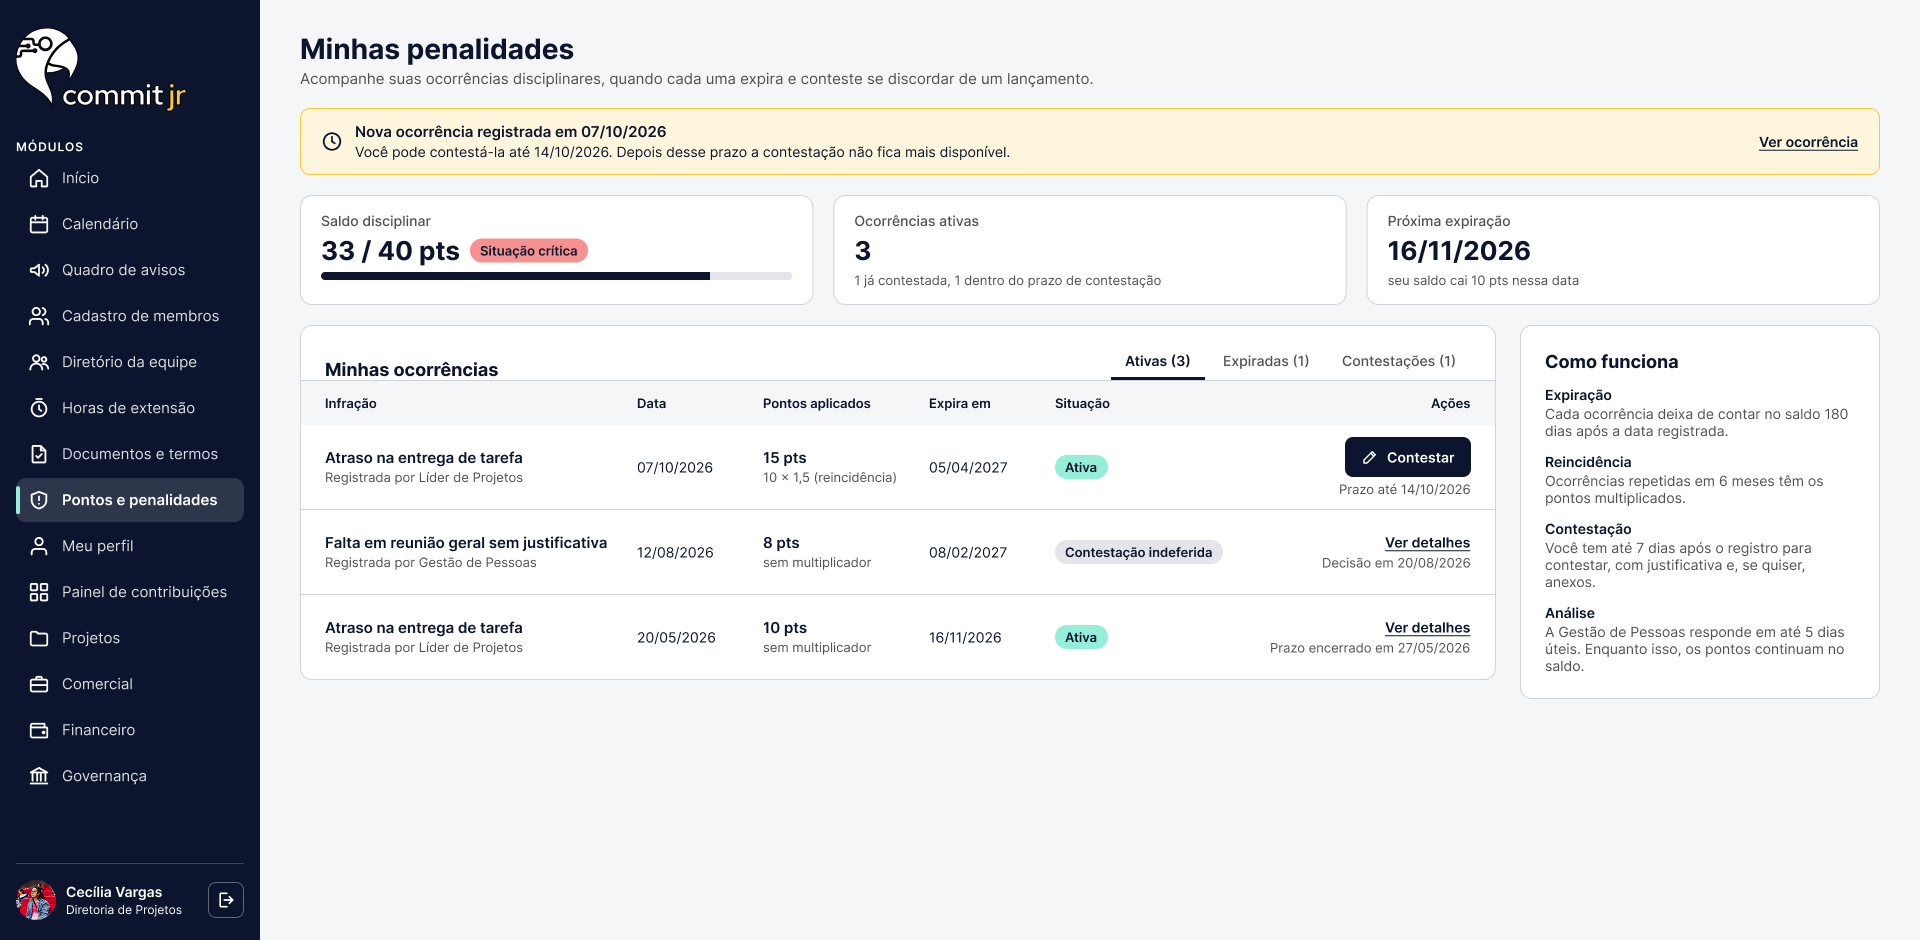
\includegraphics[width=0.88\textwidth]{Telas/pontos-membro-minhas-penalidades}} \\
\hline
\end{tabular}
\end{center}

\begin{center}
\begin{tabular}{|p{2.0cm}|p{11.5cm}|}
\hline
\textbf{PT-017} & \textbf{Painel do Membro -- Contestar Ocorrência (UC-06)} \\
\hline
\multicolumn{2}{|c|}{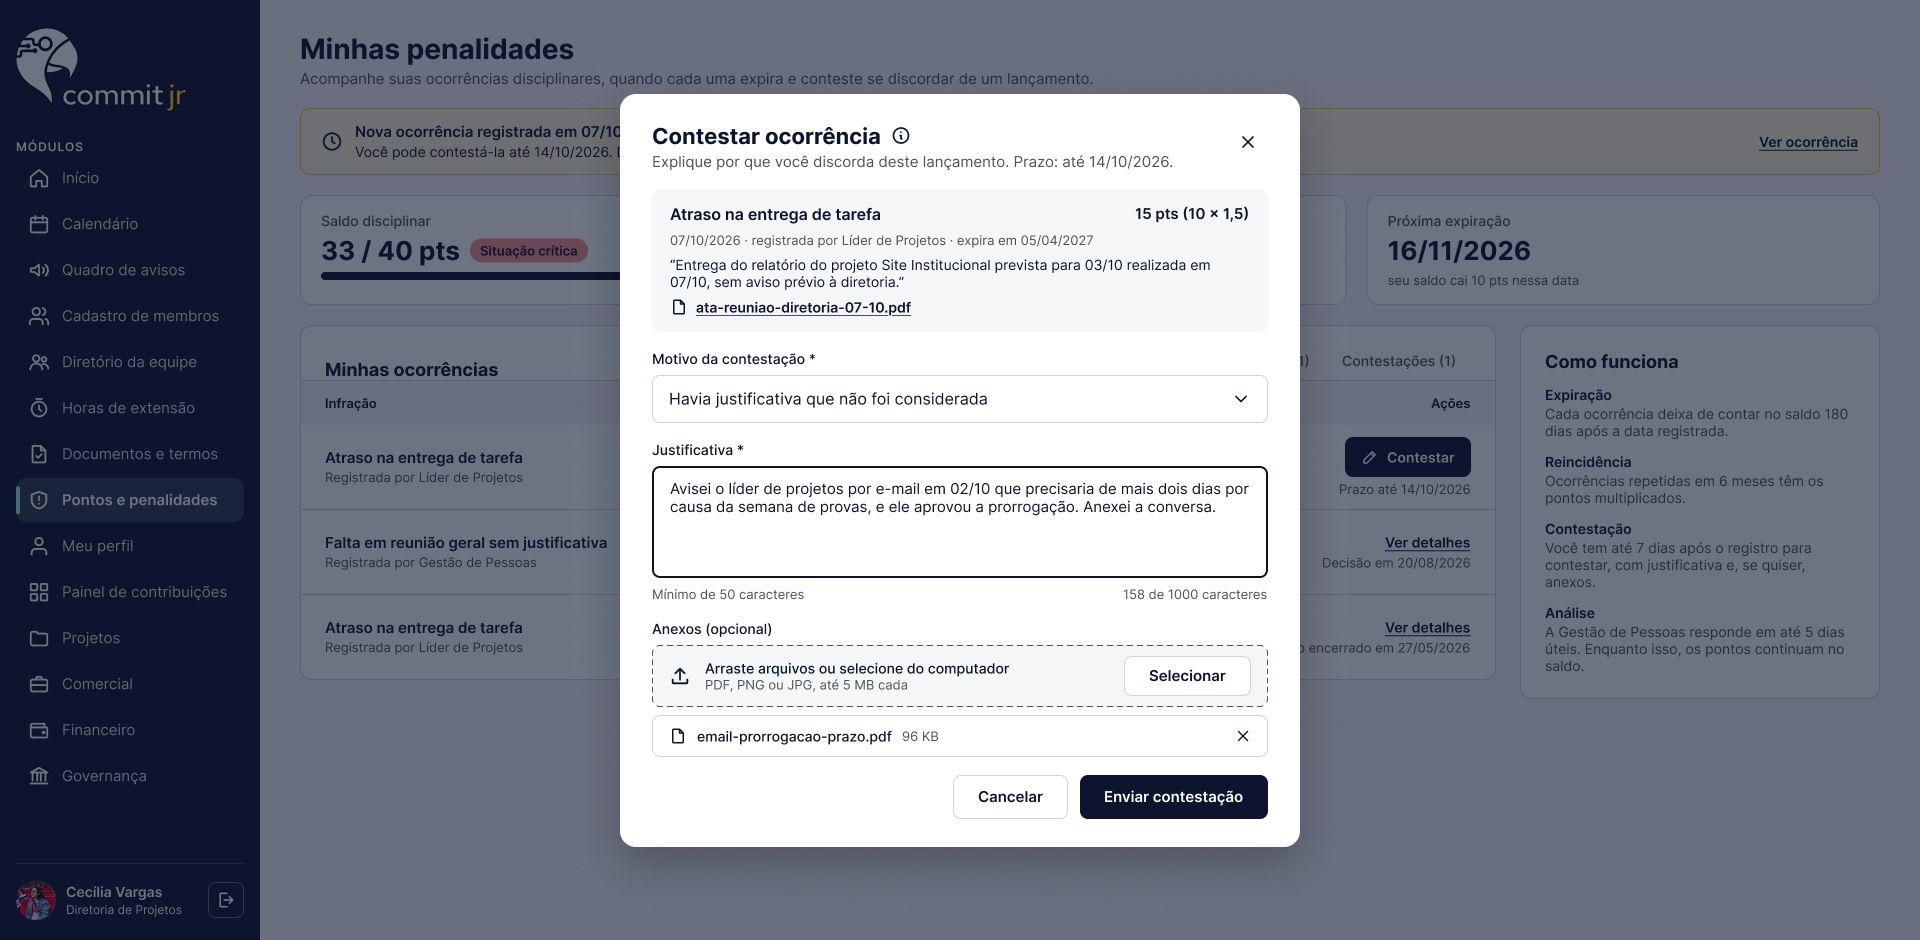
\includegraphics[width=0.88\textwidth]{Telas/pontos-membro-contestar-ocorrencia}} \\
\hline
\end{tabular}
\end{center}

\begin{center}
\begin{tabular}{|p{2.0cm}|p{11.5cm}|}
\hline
\textbf{PT-018} & \textbf{Painel do Membro -- Contestação Enviada (UC-06)} \\
\hline
\multicolumn{2}{|c|}{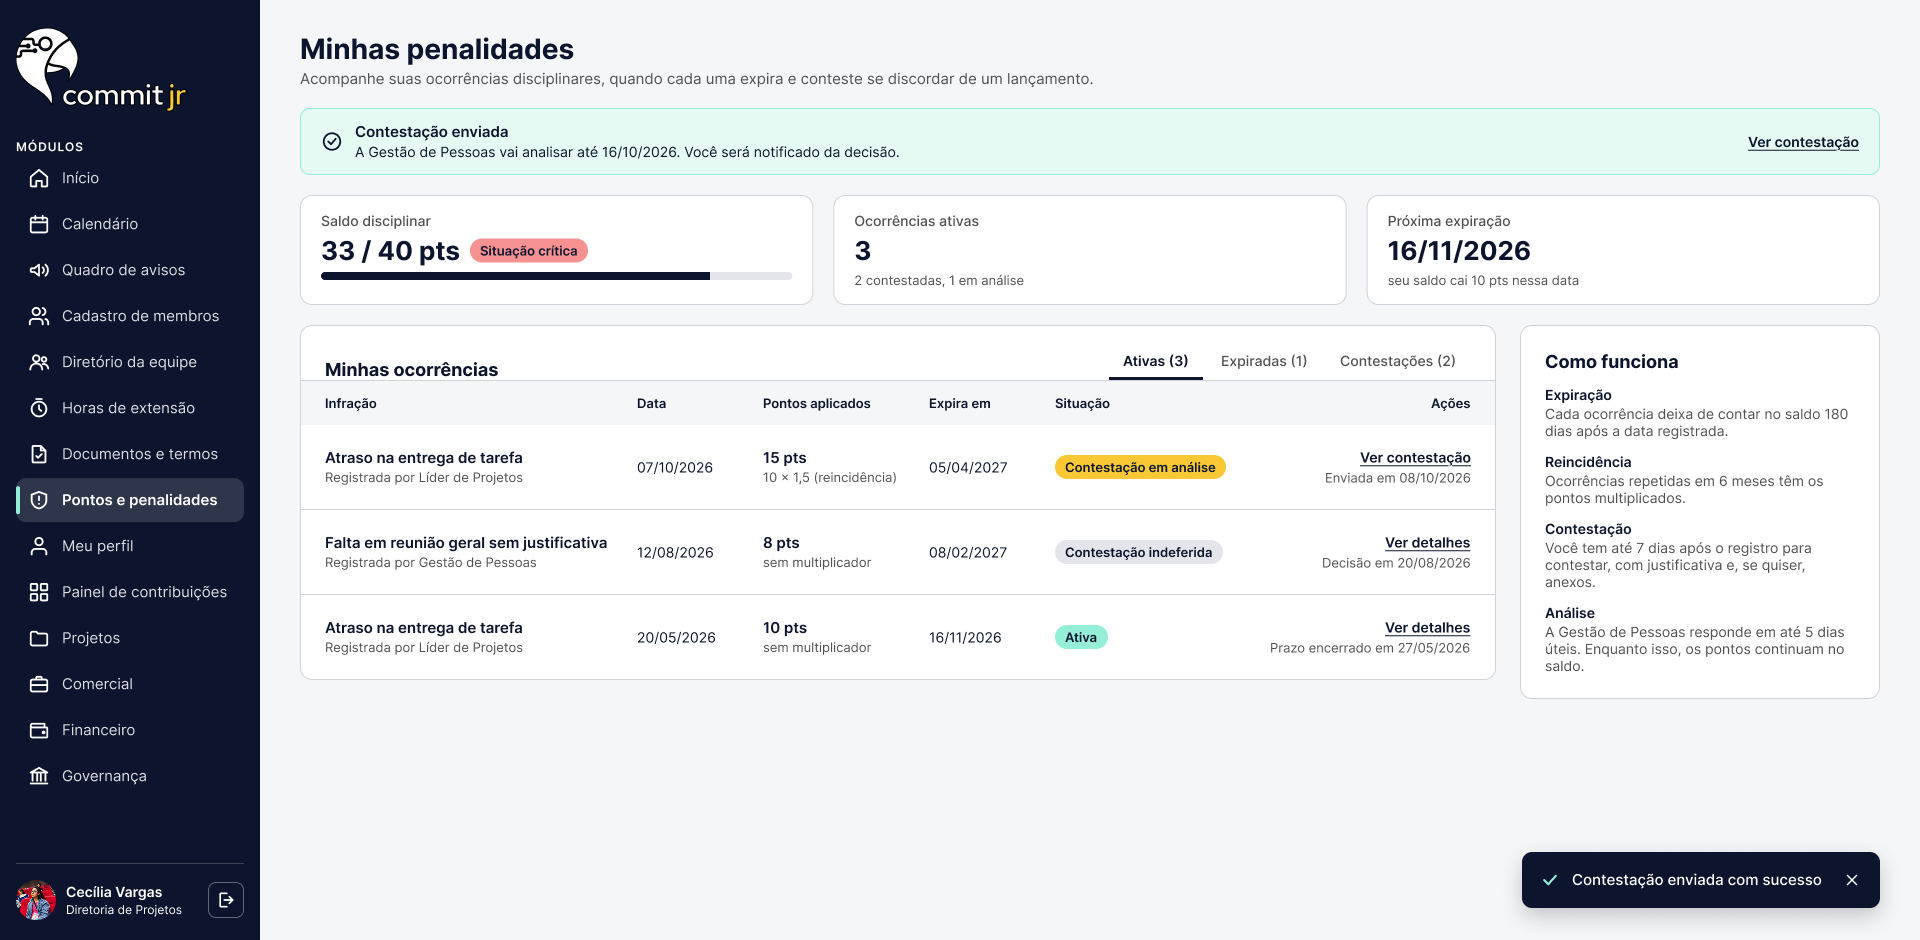
\includegraphics[width=0.88\textwidth]{Telas/pontos-membro-contestacao-enviada}} \\
\hline
\end{tabular}
\end{center}

\begin{center}
\begin{tabular}{|p{2.0cm}|p{11.5cm}|}
\hline
\textbf{PT-019} & \textbf{Quadro de Avisos -- Publicar Aviso (UC-10)} \\
\hline
\multicolumn{2}{|c|}{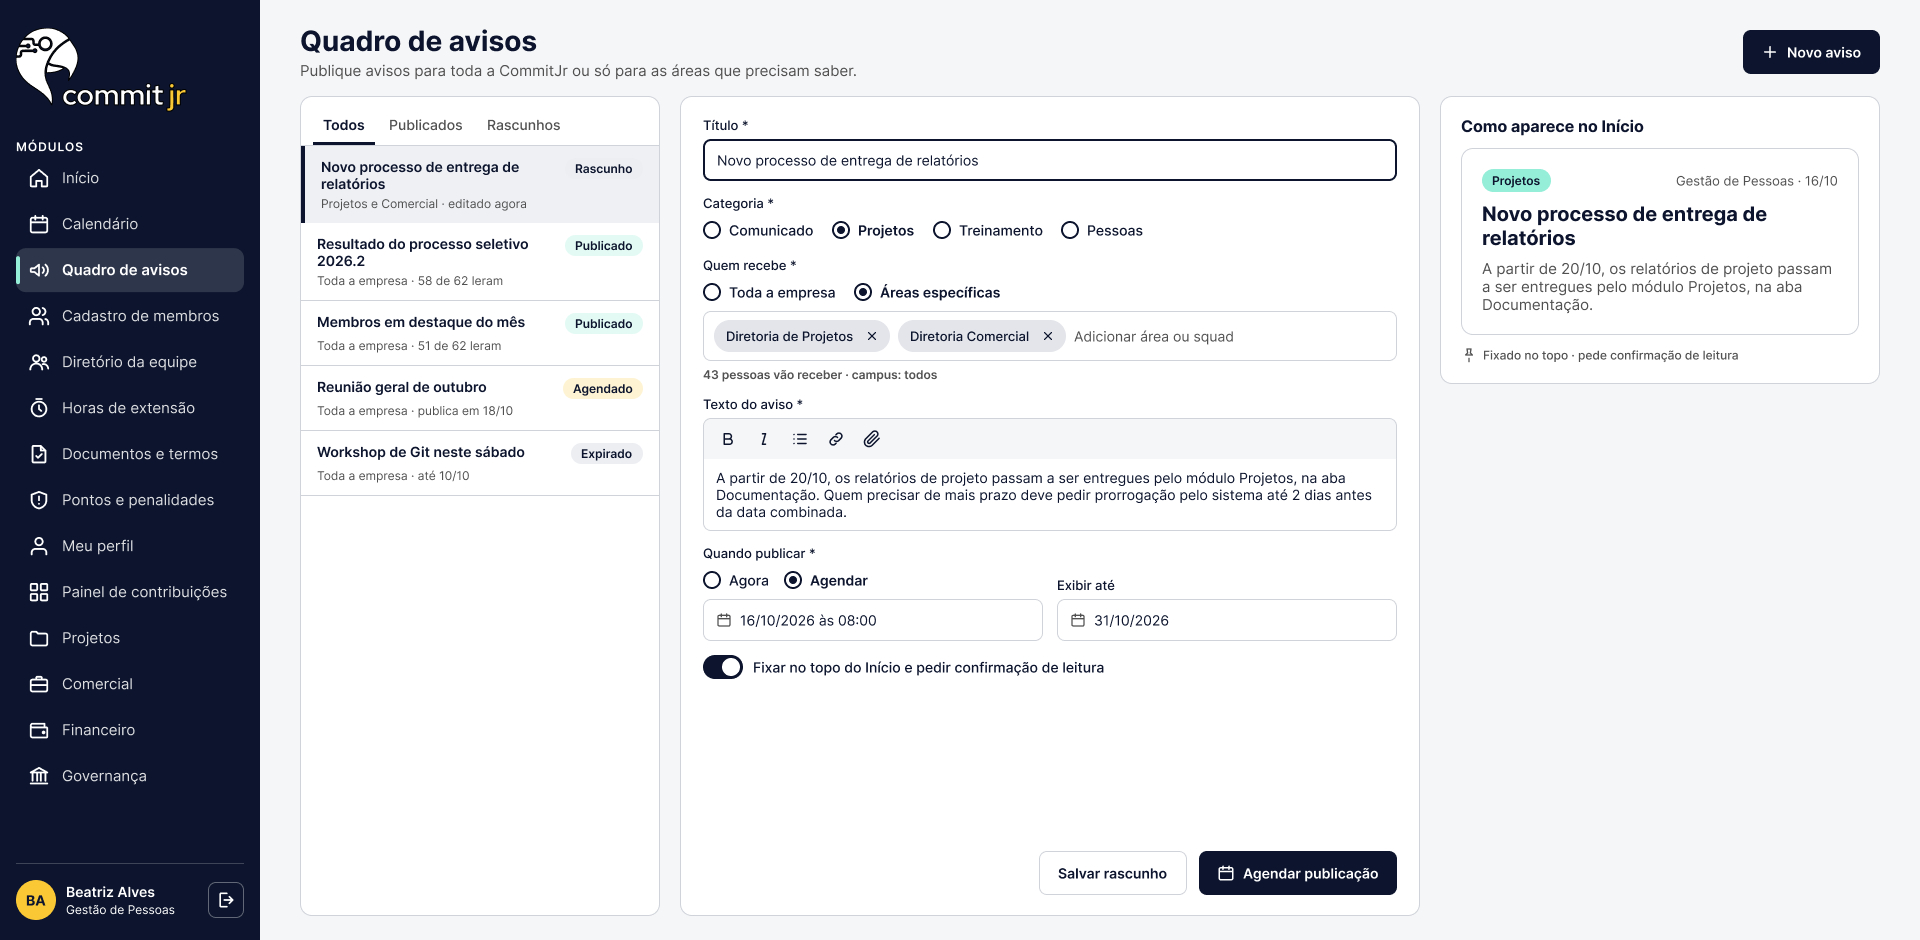
\includegraphics[width=0.88\textwidth]{Telas/quadro-avisos-publicar}} \\
\hline
\end{tabular}
\end{center}

\begin{center}
\begin{tabular}{|p{2.0cm}|p{11.5cm}|}
\hline
\textbf{PT-020} & \textbf{Calendário Corporativo -- Visão Mensal (UC-05)} \\
\hline
\multicolumn{2}{|c|}{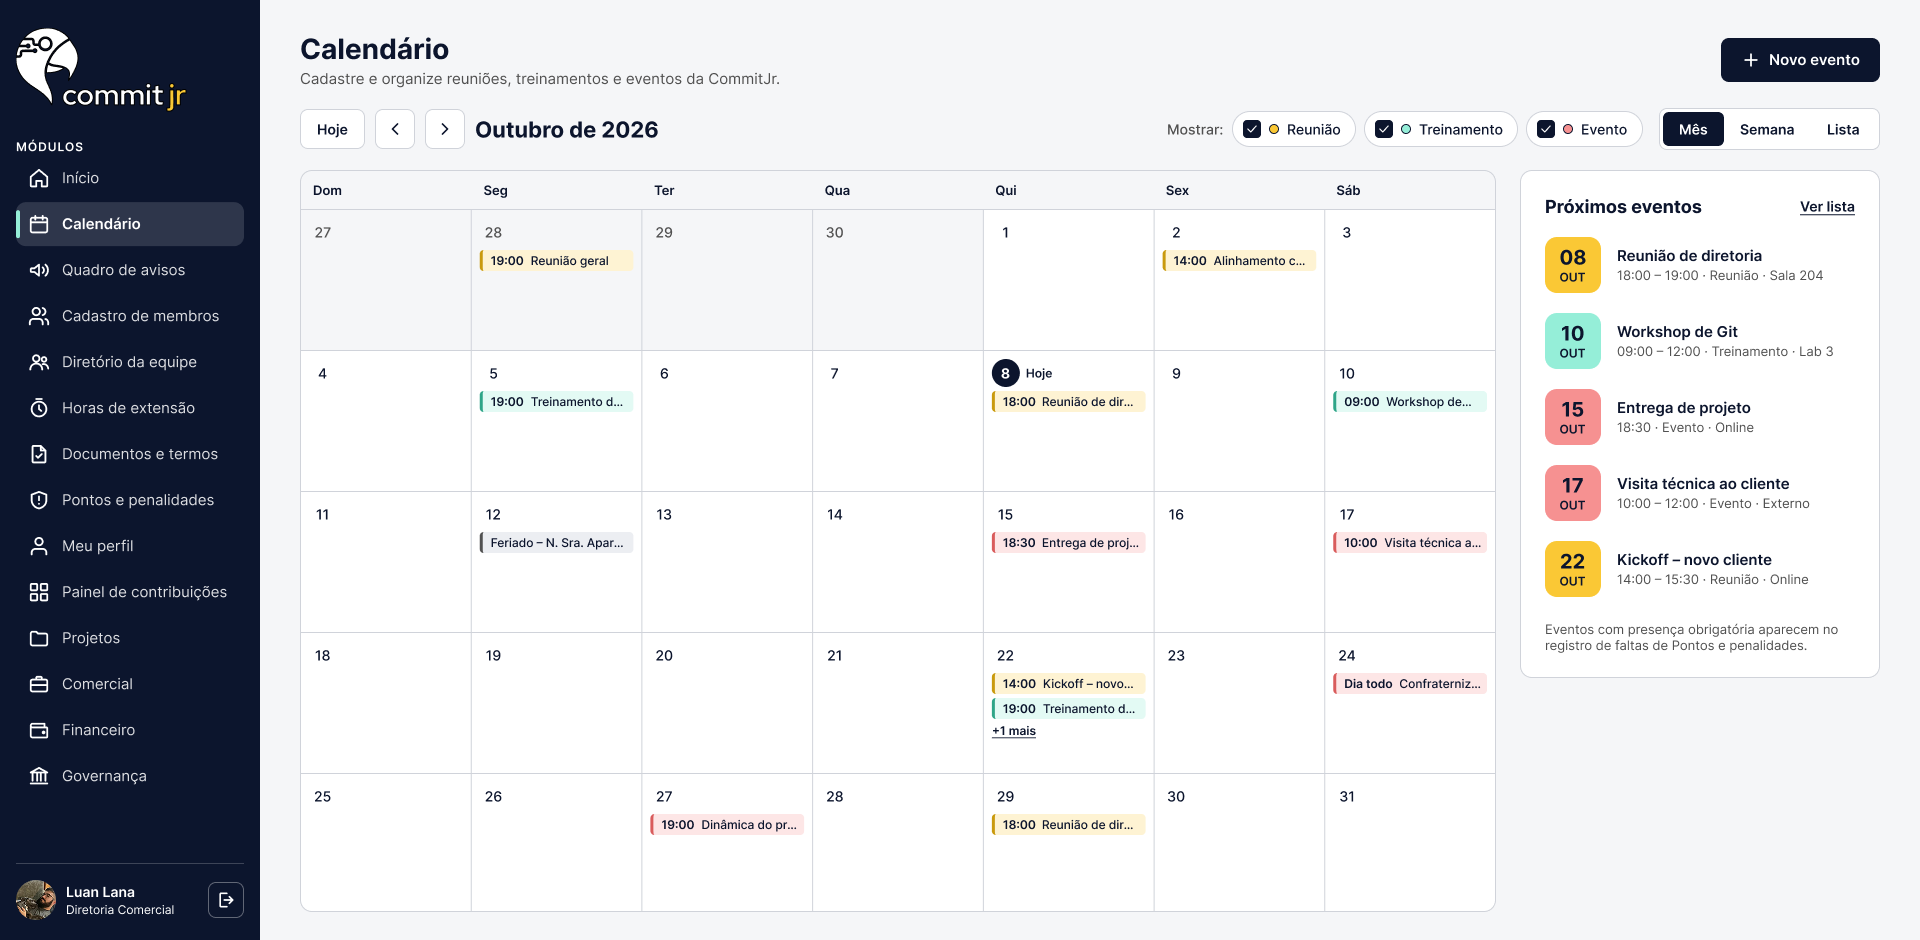
\includegraphics[width=0.88\textwidth]{Telas/calendario-visao-mensal}} \\
\hline
\end{tabular}
\end{center}

\begin{center}
\begin{tabular}{|p{2.0cm}|p{11.5cm}|}
\hline
\textbf{PT-021} & \textbf{Calendário Corporativo -- Novo Evento Institucional (UC-05)} \\
\hline
\multicolumn{2}{|c|}{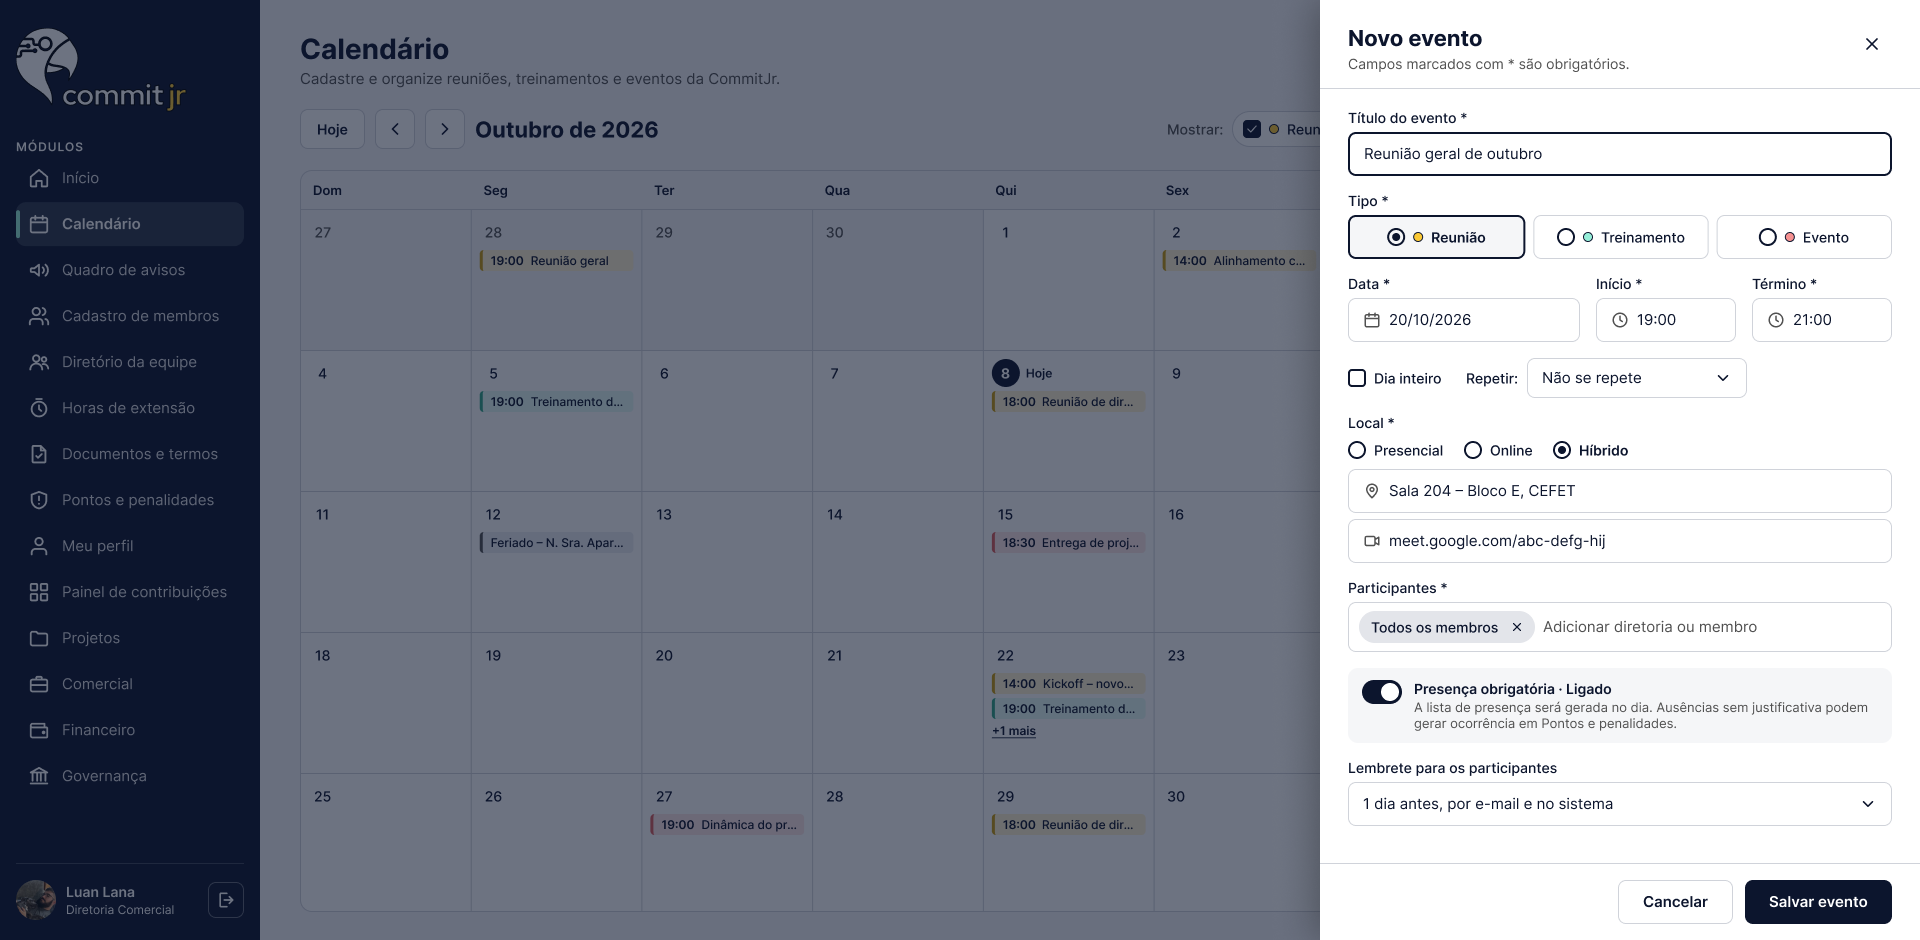
\includegraphics[width=0.88\textwidth]{Telas/calendario-novo-evento}} \\
\hline
\end{tabular}
\end{center}

\begin{center}
\begin{tabular}{|p{2.0cm}|p{11.5cm}|}
\hline
\textbf{PT-022} & \textbf{Calendário Corporativo -- Agendar Reunião 1-on-1 (UC-05)} \\
\hline
\multicolumn{2}{|c|}{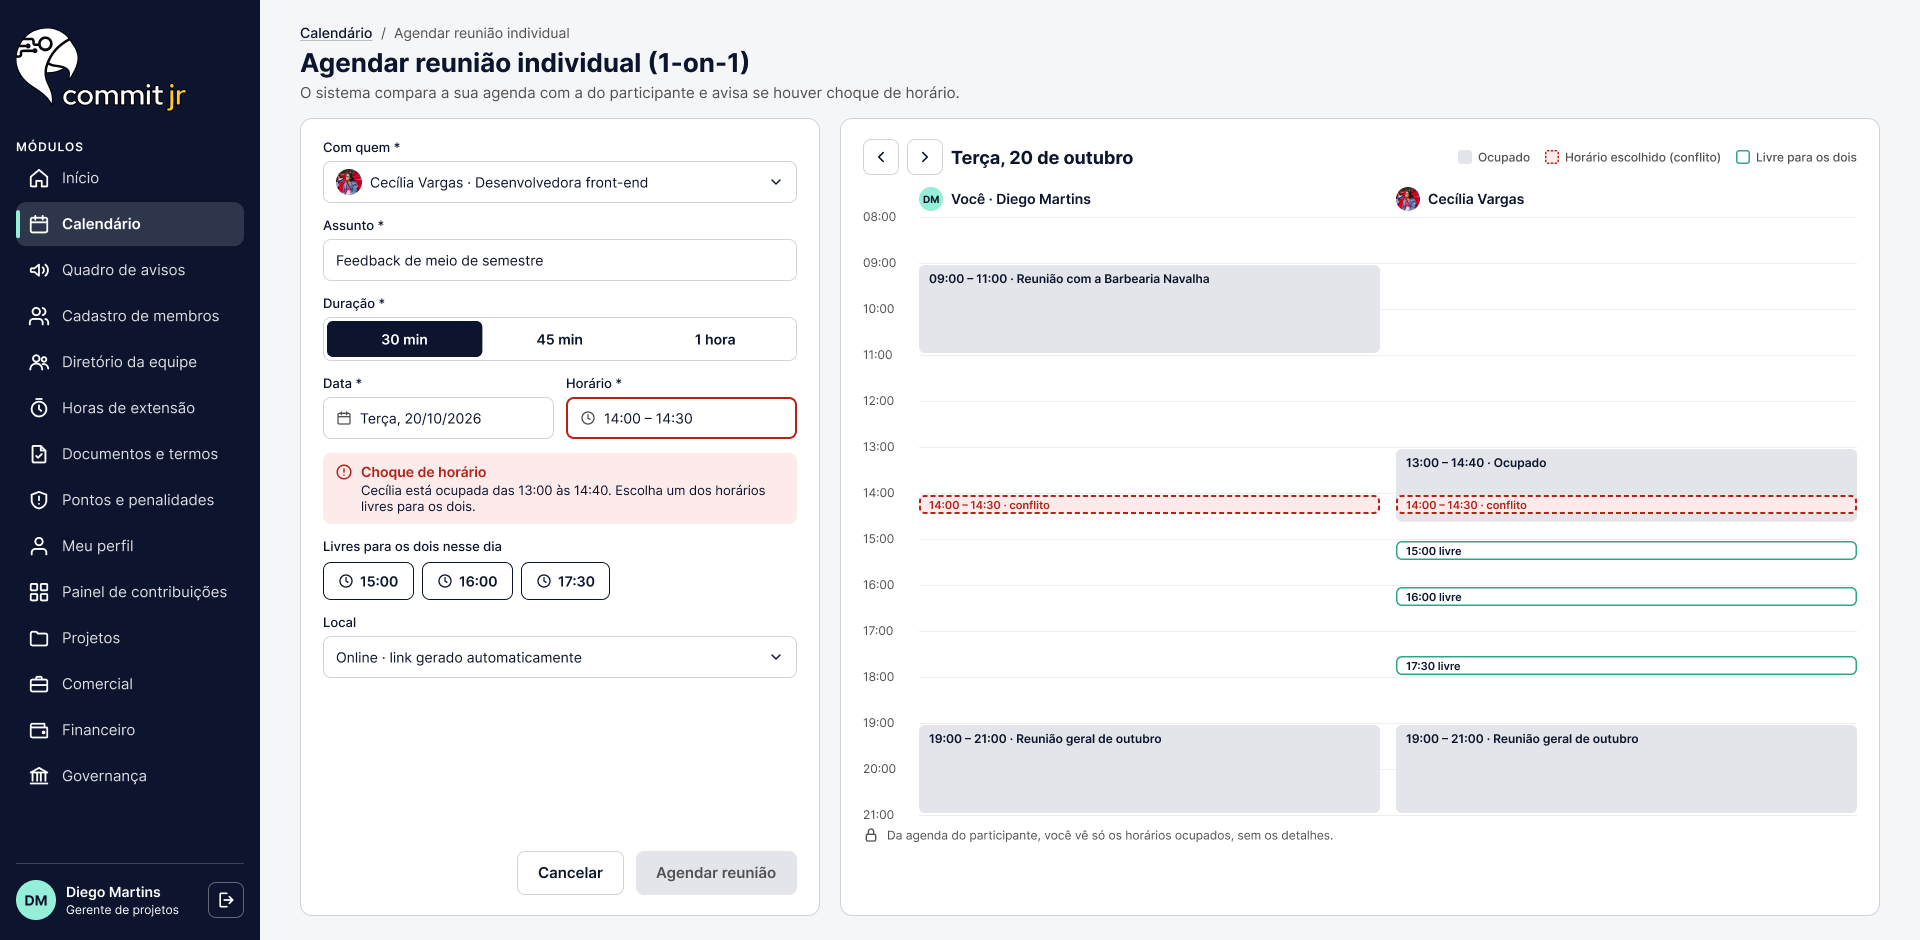
\includegraphics[width=0.88\textwidth]{Telas/calendario-agendar-1on1}} \\
\hline
\end{tabular}
\end{center}

\begin{center}
\begin{tabular}{|p{2.0cm}|p{11.5cm}|}
\hline
\textbf{PT-023} & \textbf{Calendário Corporativo -- Confirmação de Evento Salvo (UC-05)} \\
\hline
\multicolumn{2}{|c|}{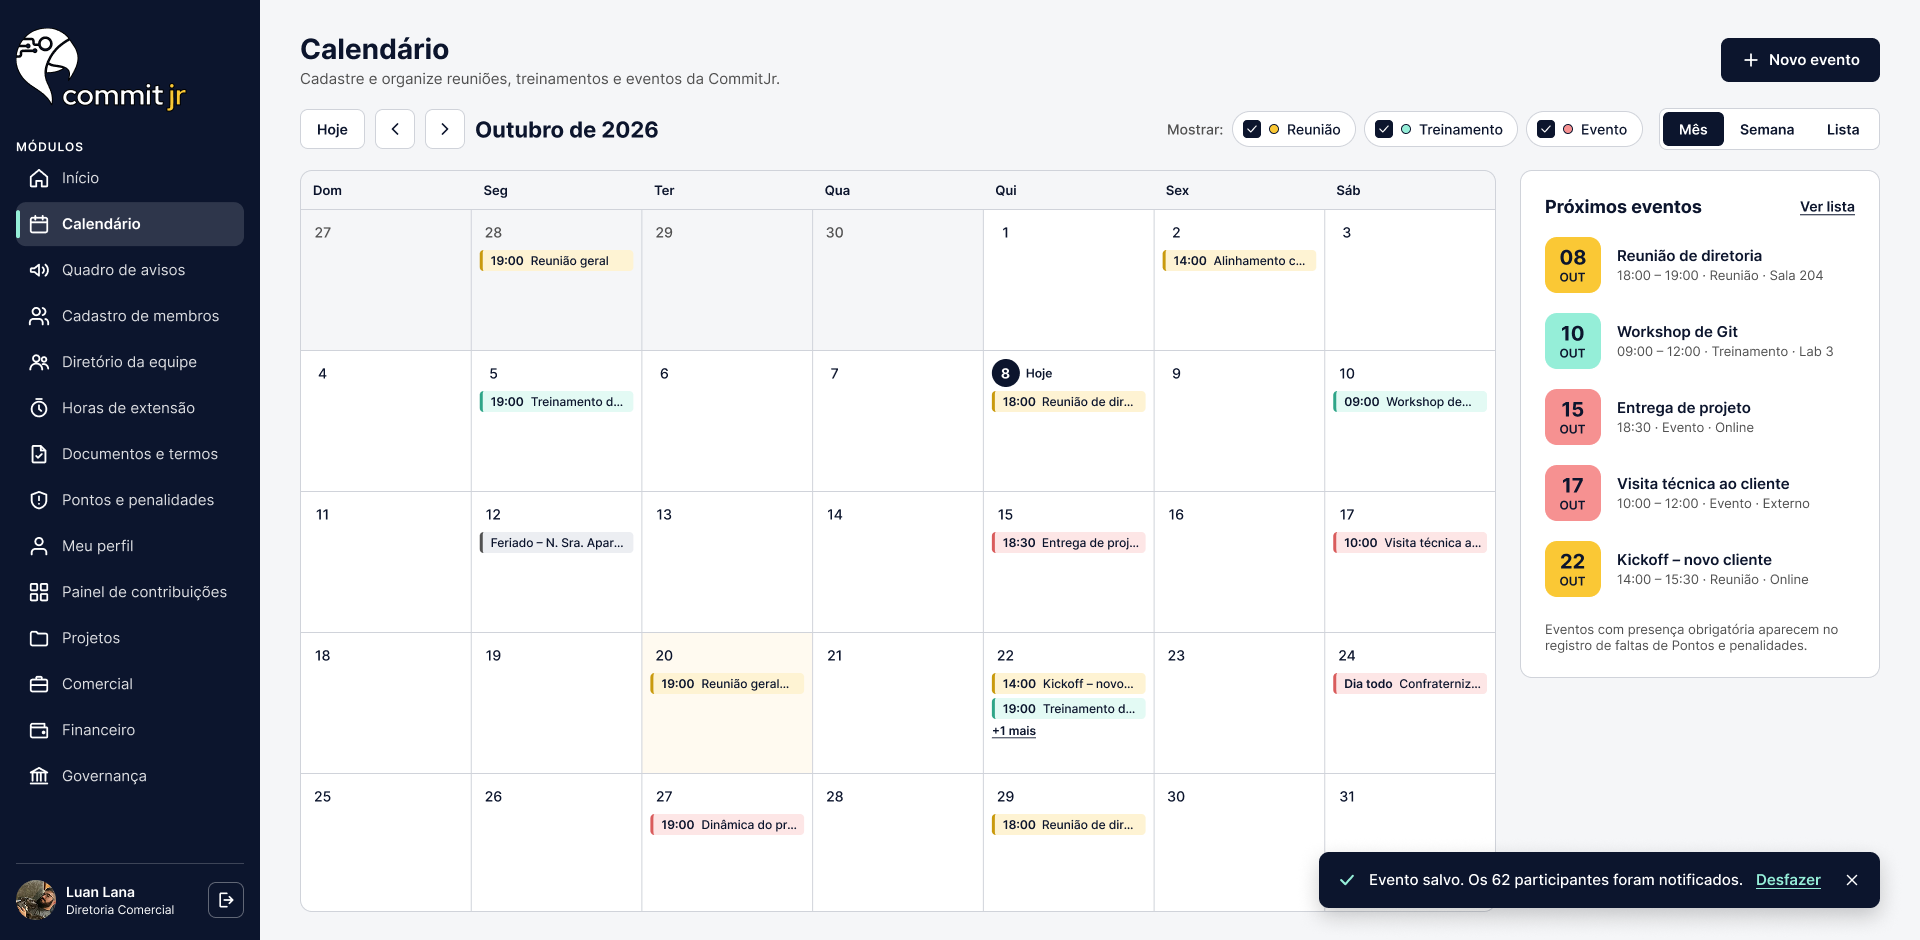
\includegraphics[width=0.88\textwidth]{Telas/calendario-evento-salvo}} \\
\hline
\end{tabular}
\end{center}

\begin{center}
\begin{tabular}{|p{2.0cm}|p{11.5cm}|}
\hline
\textbf{PT-024} & \textbf{Governança -- Perfis de Acesso e Propostas (UC-18)} \\
\hline
\multicolumn{2}{|c|}{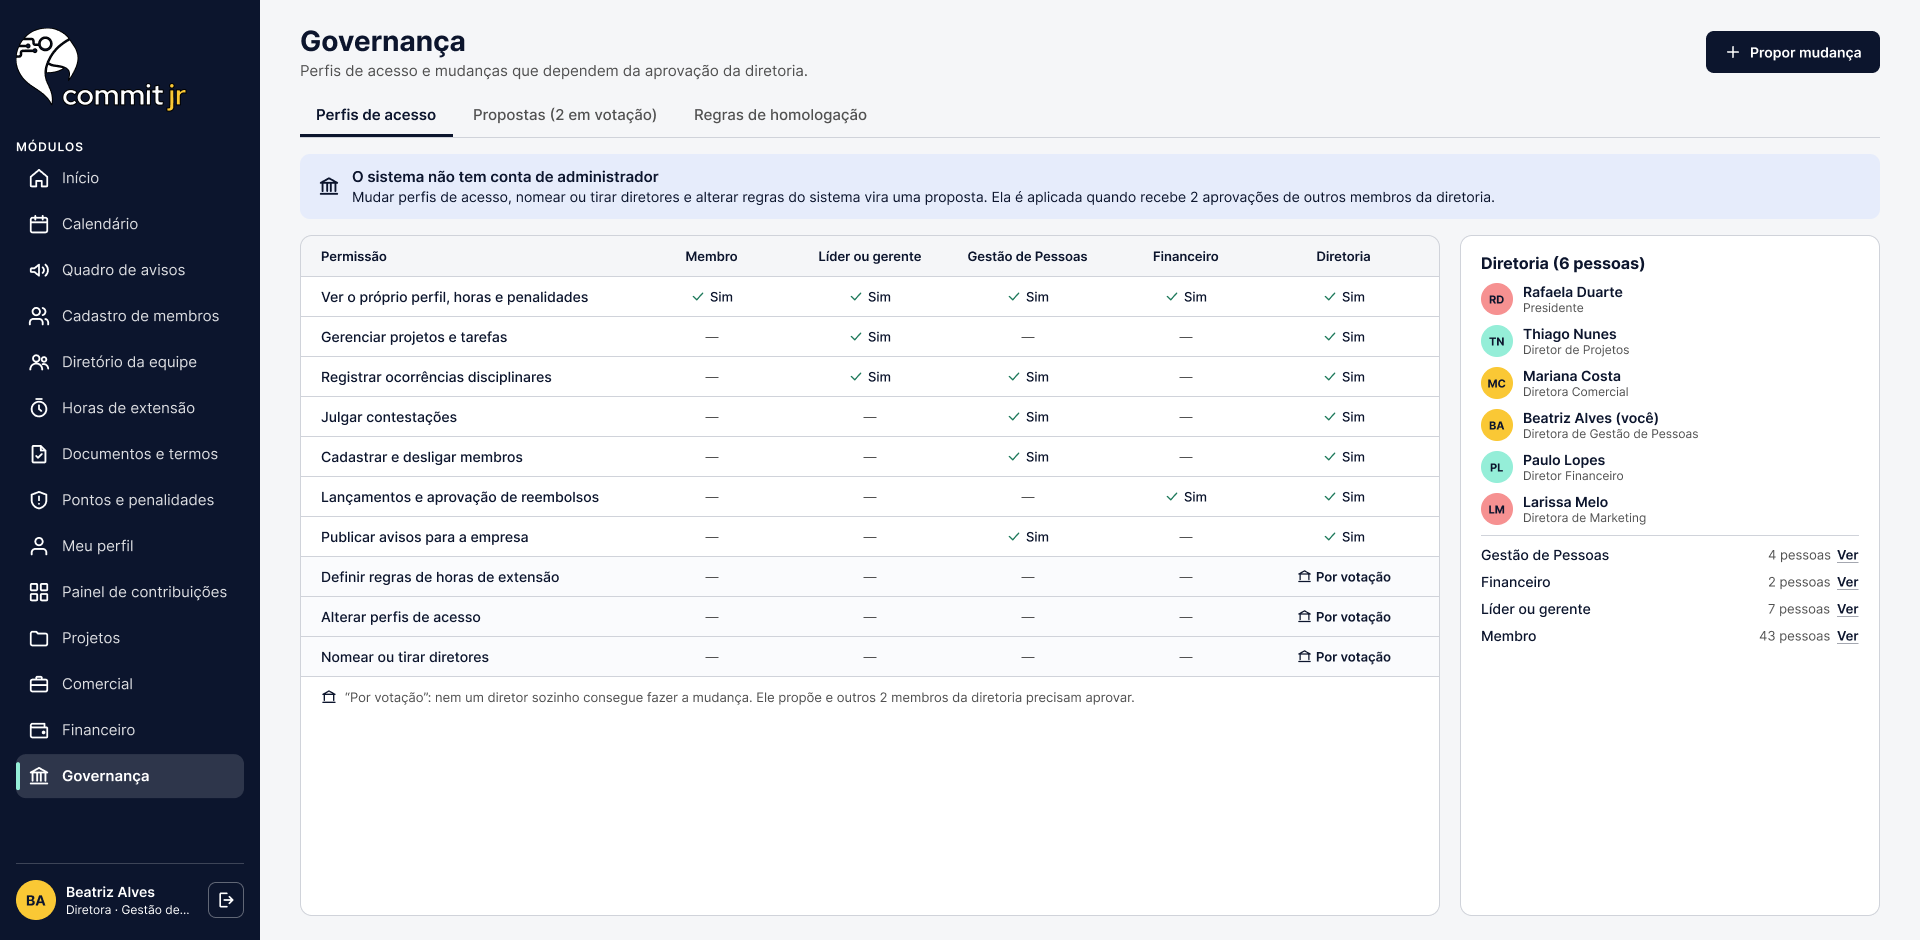
\includegraphics[width=0.88\textwidth]{Telas/governanca-perfis-acesso}} \\
\hline
\end{tabular}
\end{center}

\begin{center}
\begin{tabular}{|p{2.0cm}|p{11.5cm}|}
\hline
\textbf{PT-025} & \textbf{Governança -- Homologar Proposta (UC-19)} \\
\hline
\multicolumn{2}{|c|}{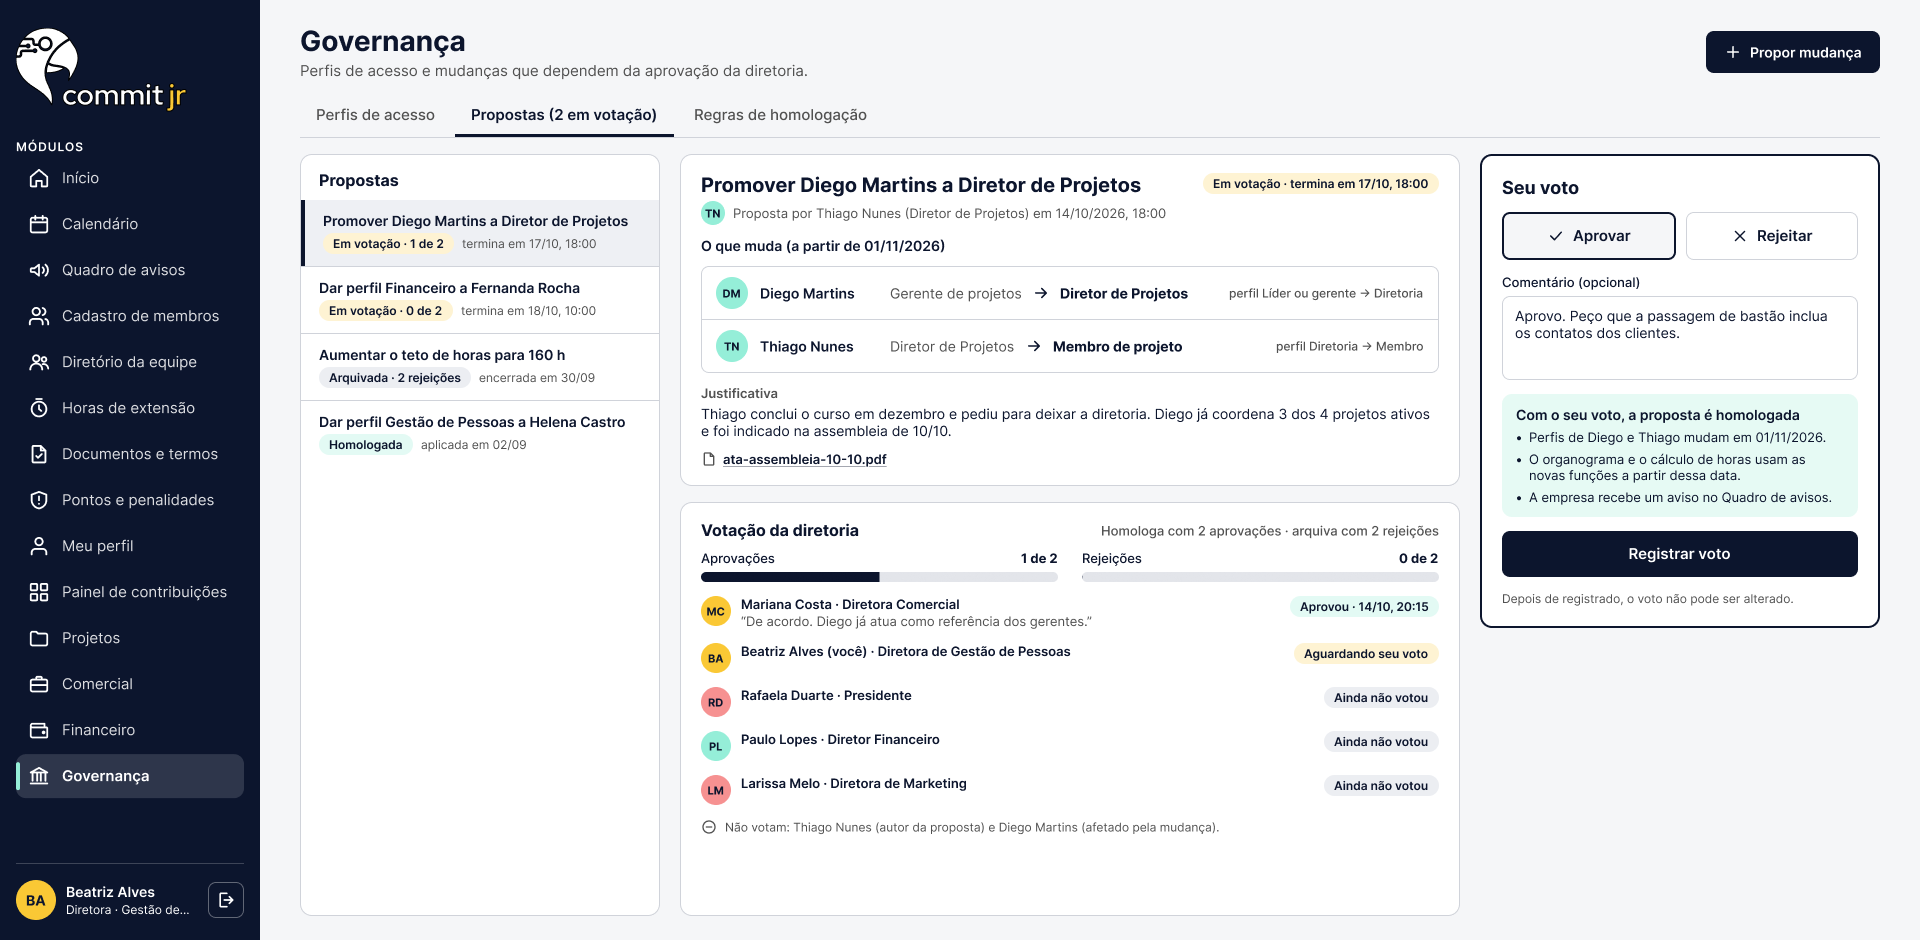
\includegraphics[width=0.88\textwidth]{Telas/governanca-homologar-proposta}} \\
\hline
\end{tabular}
\end{center}

\begin{center}
\begin{tabular}{|p{2.0cm}|p{11.5cm}|}
\hline
\textbf{PT-026} & \textbf{Projetos -- Visão do Gerente (UC-17)} \\
\hline
\multicolumn{2}{|c|}{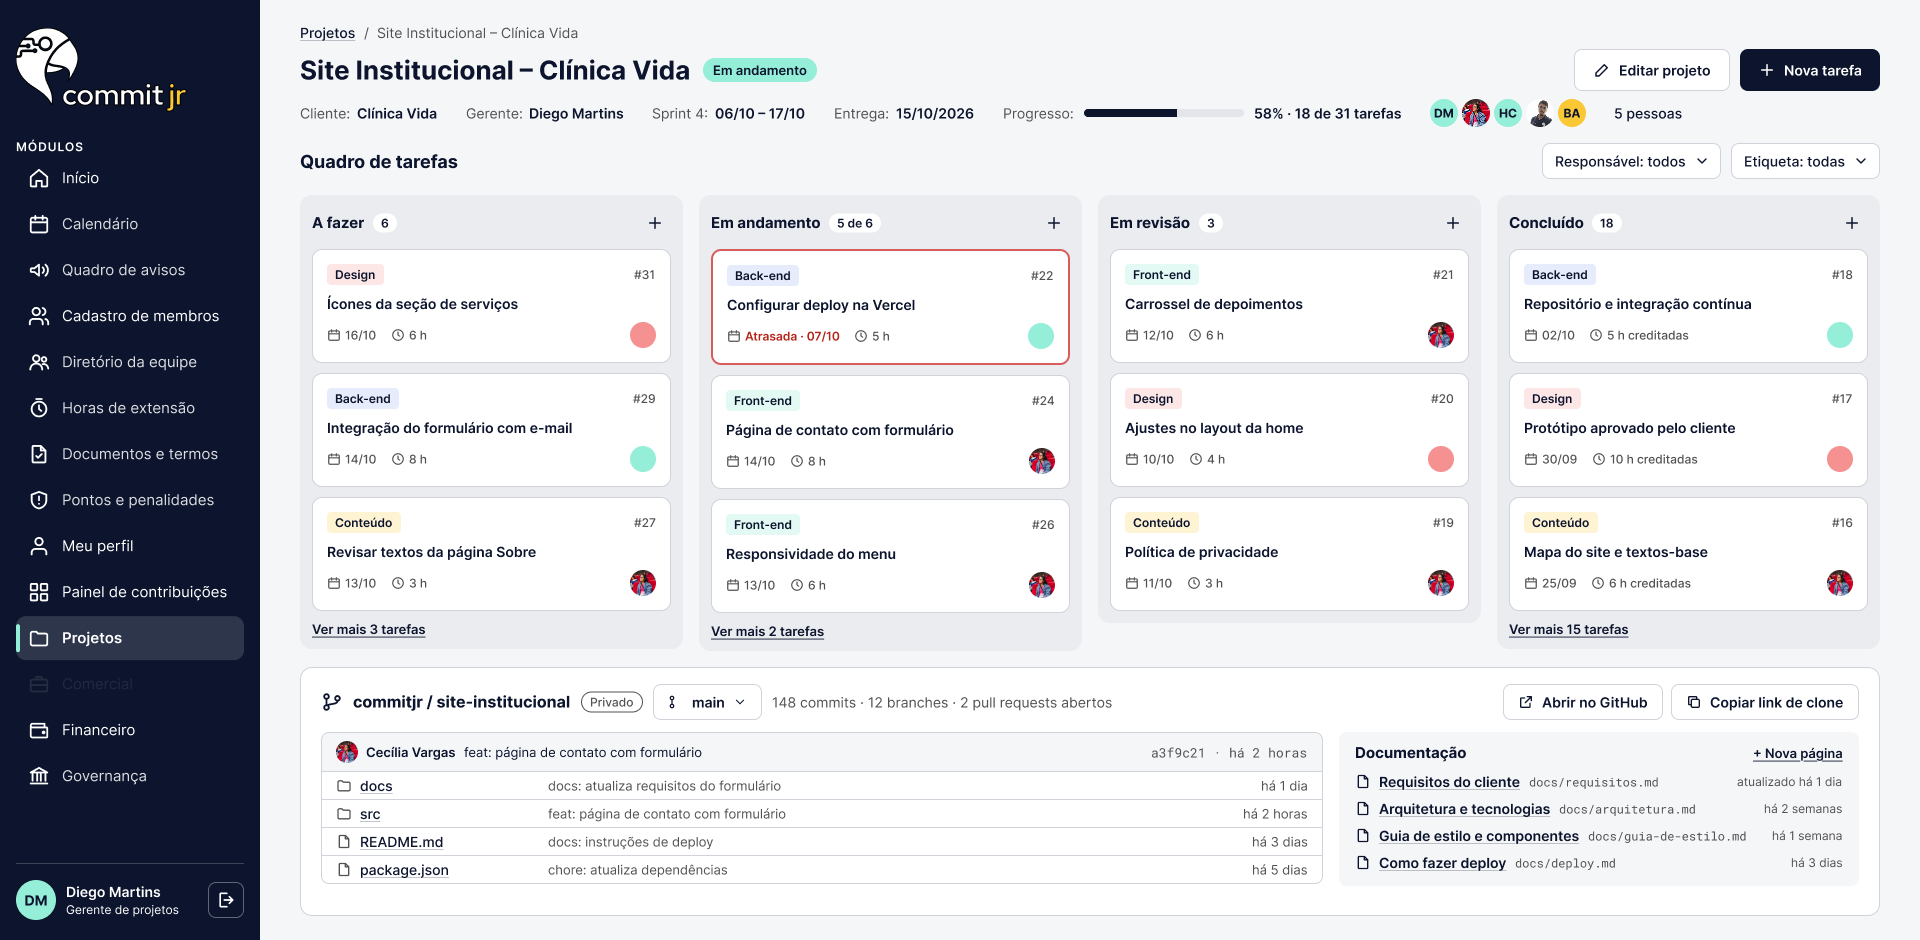
\includegraphics[width=0.88\textwidth]{Telas/projetos-visao-gerente}} \\
\hline
\end{tabular}
\end{center}

\begin{center}
\begin{tabular}{|p{2.0cm}|p{11.5cm}|}
\hline
\textbf{PT-027} & \textbf{Projetos -- Lista Geral (Gerente) (UC-17)} \\
\hline
\multicolumn{2}{|c|}{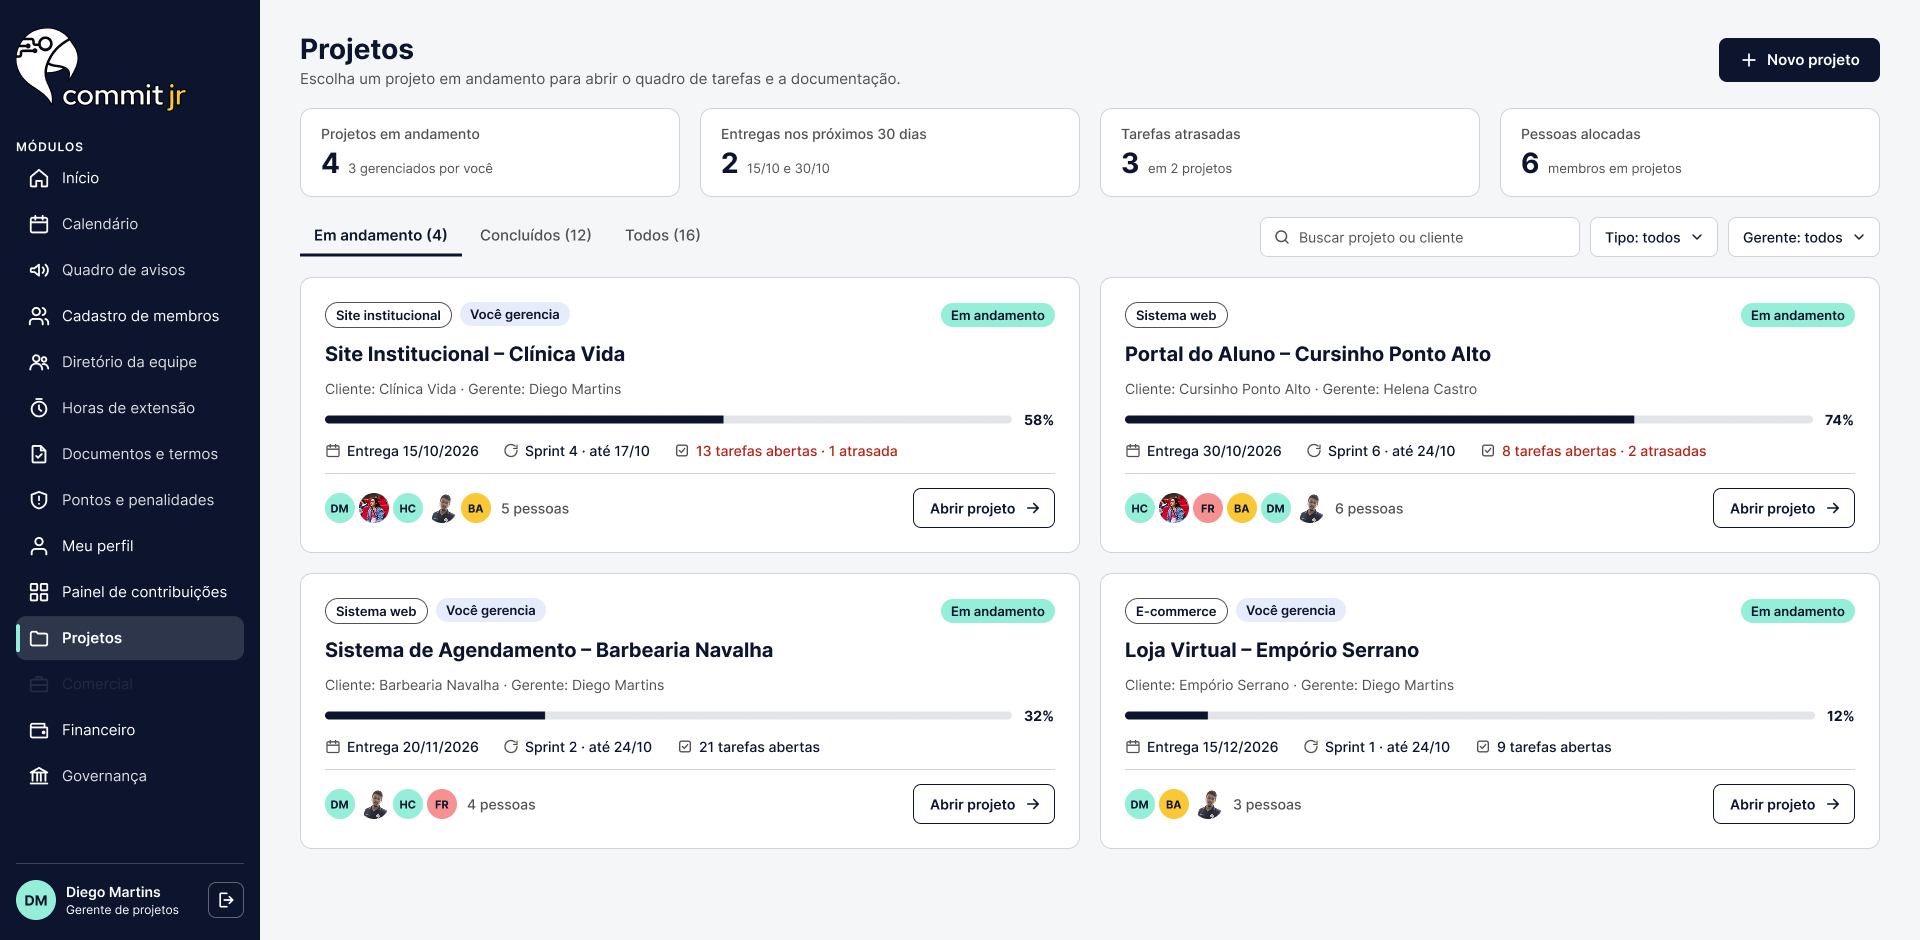
\includegraphics[width=0.88\textwidth]{Telas/projetos-lista-gerente}} \\
\hline
\end{tabular}
\end{center}

\begin{center}
\begin{tabular}{|p{2.0cm}|p{11.5cm}|}
\hline
\textbf{PT-028} & \textbf{Projetos -- Visão do Membro (UC-07)} \\
\hline
\multicolumn{2}{|c|}{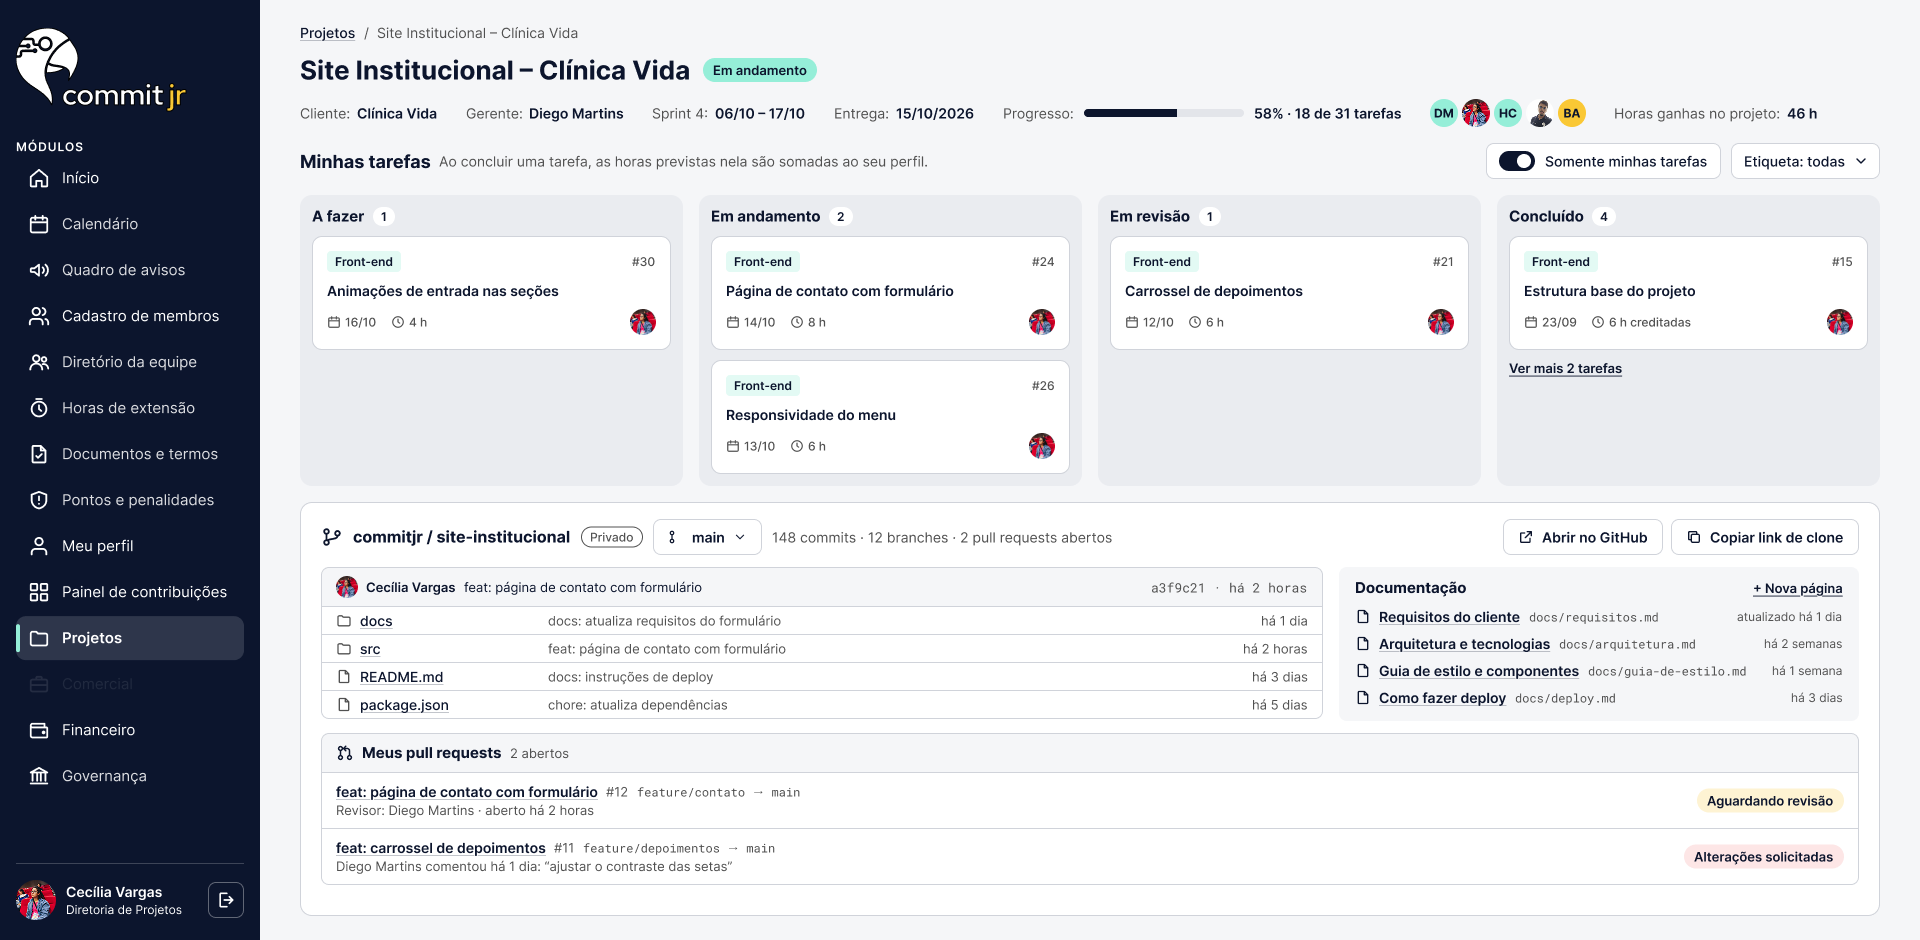
\includegraphics[width=0.88\textwidth]{Telas/projetos-visao-membro}} \\
\hline
\end{tabular}
\end{center}

\begin{center}
\begin{tabular}{|p{2.0cm}|p{11.5cm}|}
\hline
\textbf{PT-029} & \textbf{Projetos -- Lista de Tarefas do Membro (UC-07)} \\
\hline
\multicolumn{2}{|c|}{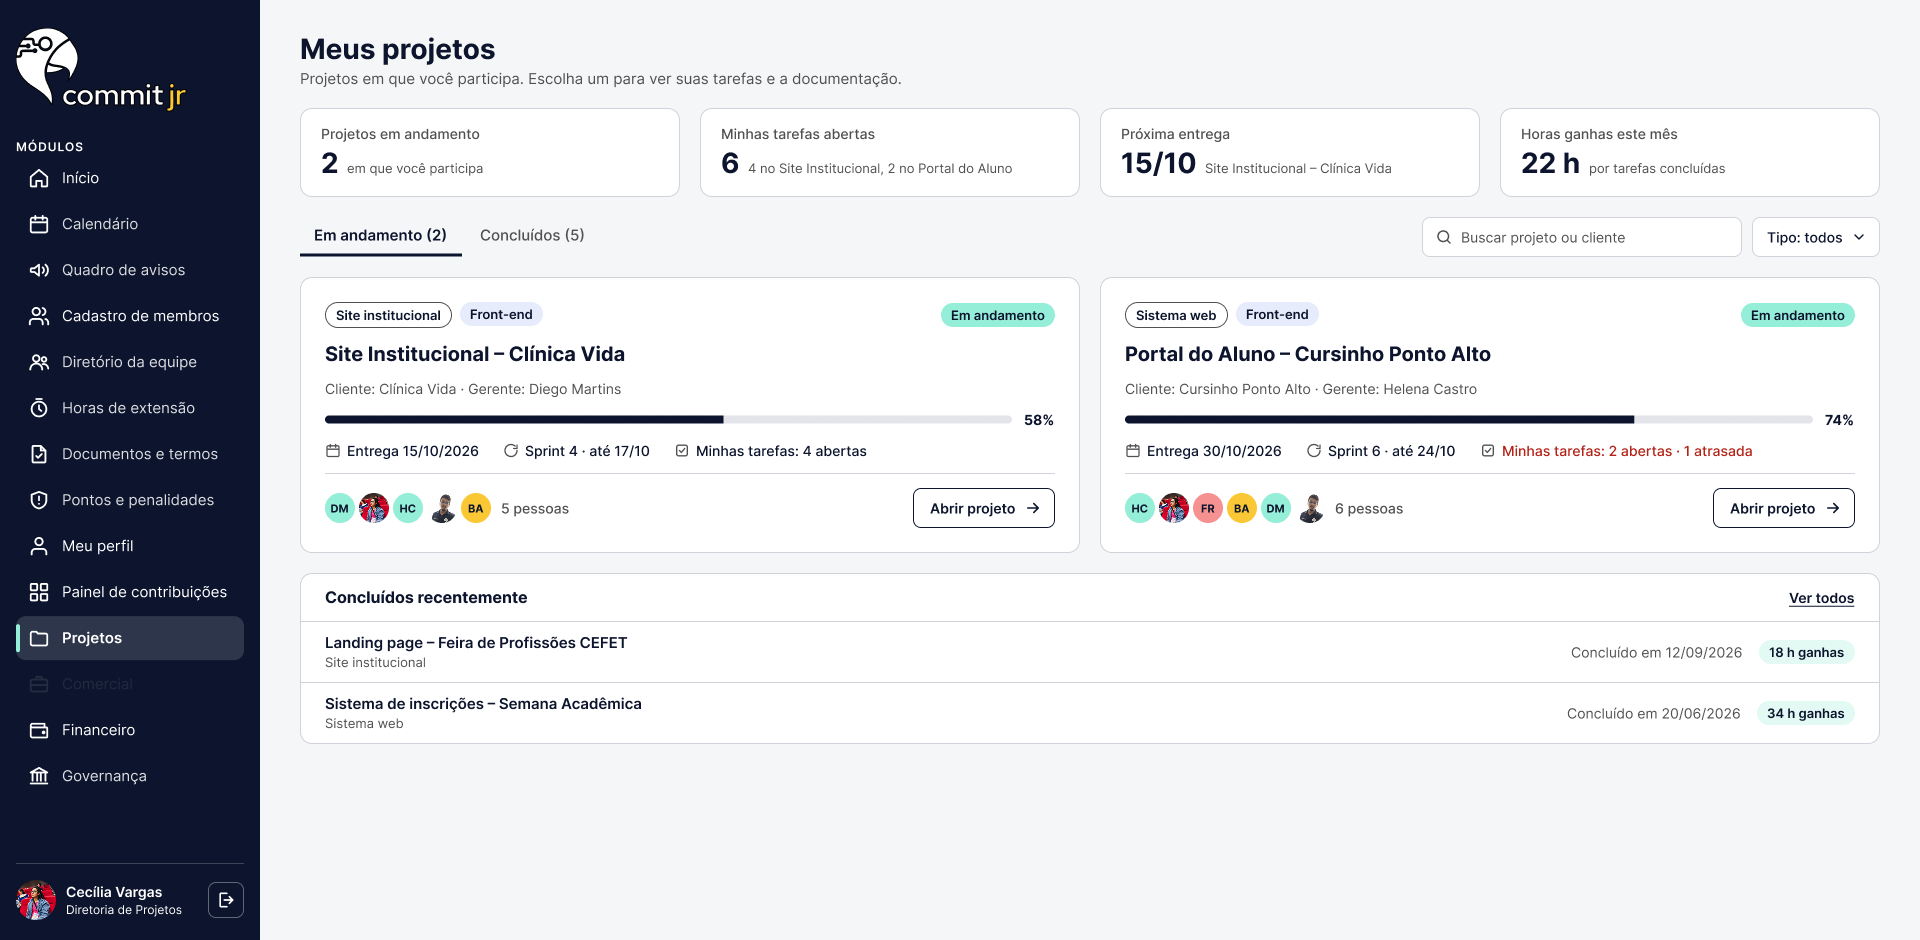
\includegraphics[width=0.88\textwidth]{Telas/projetos-lista-membro}} \\
\hline
\end{tabular}
\end{center}

\begin{center}
\begin{tabular}{|p{2.0cm}|p{11.5cm}|}
\hline
\textbf{PT-030} & \textbf{Projetos -- Cadastro de Nova Tarefa (UC-17)} \\
\hline
\multicolumn{2}{|c|}{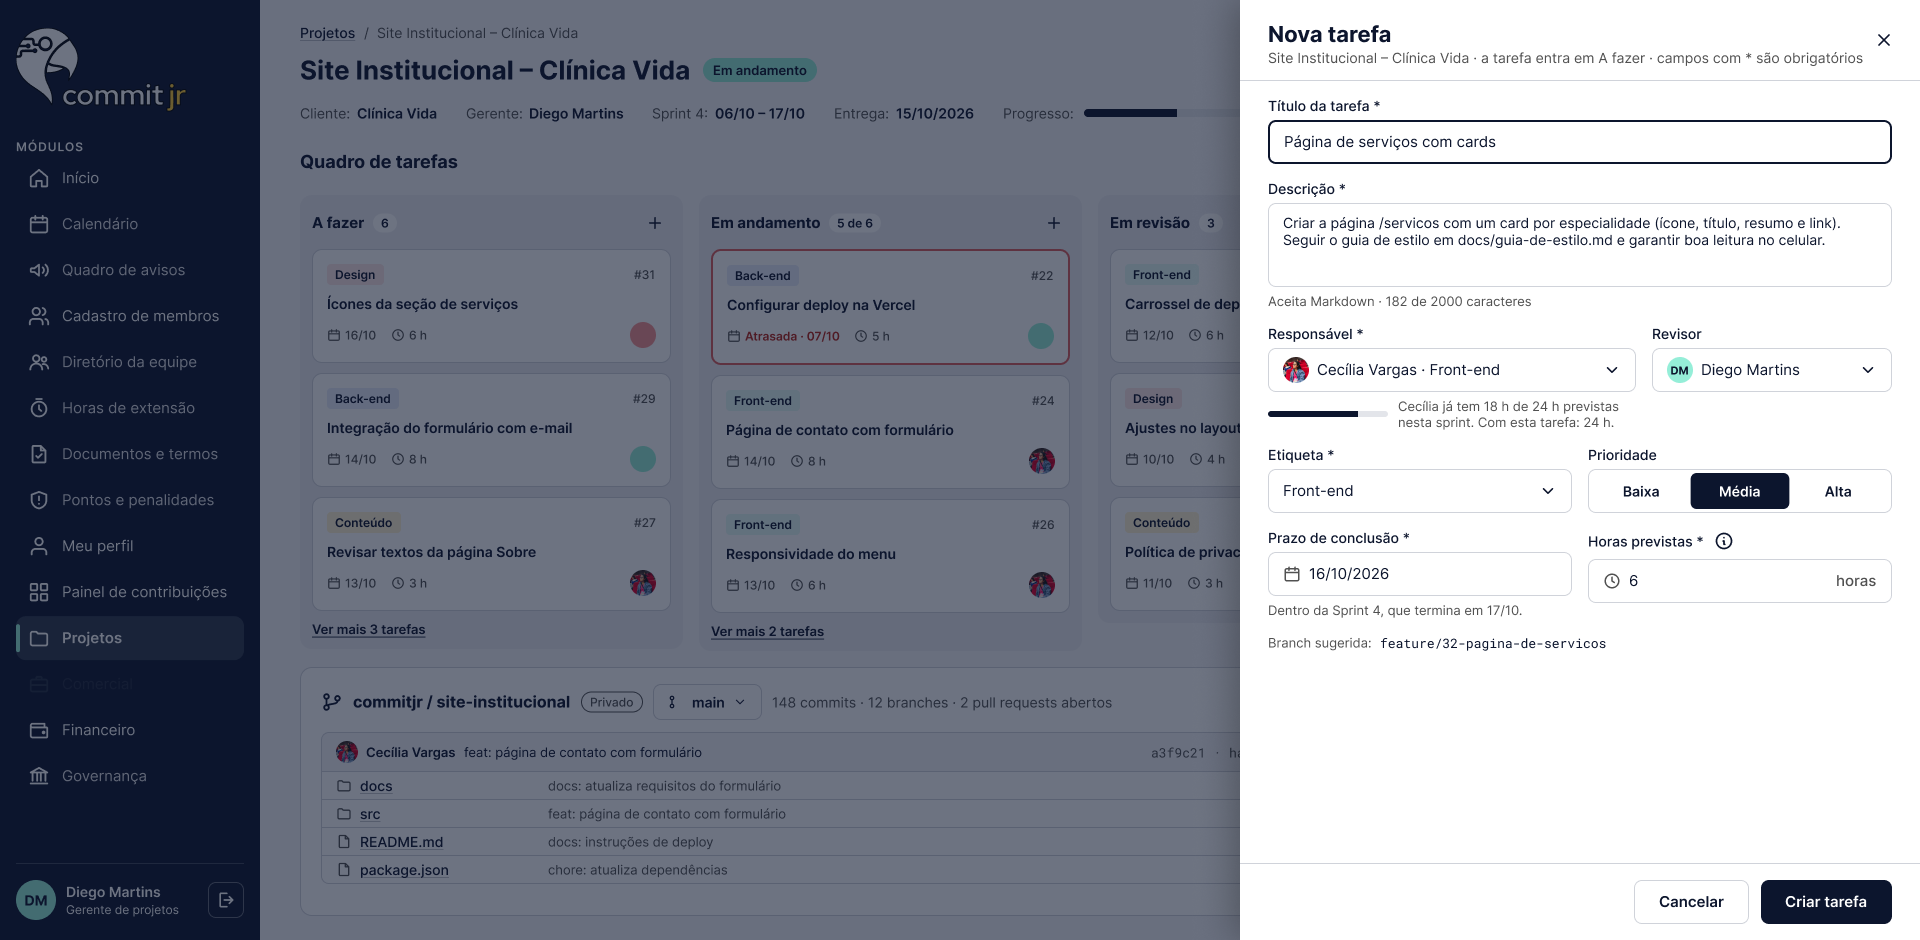
\includegraphics[width=0.88\textwidth]{Telas/projetos-nova-tarefa}} \\
\hline
\end{tabular}
\end{center}

\begin{center}
\begin{tabular}{|p{2.0cm}|p{11.5cm}|}
\hline
\textbf{PT-031} & \textbf{Comercial -- Cadastro e Consulta de Clientes (UC-16)} \\
\hline
\multicolumn{2}{|c|}{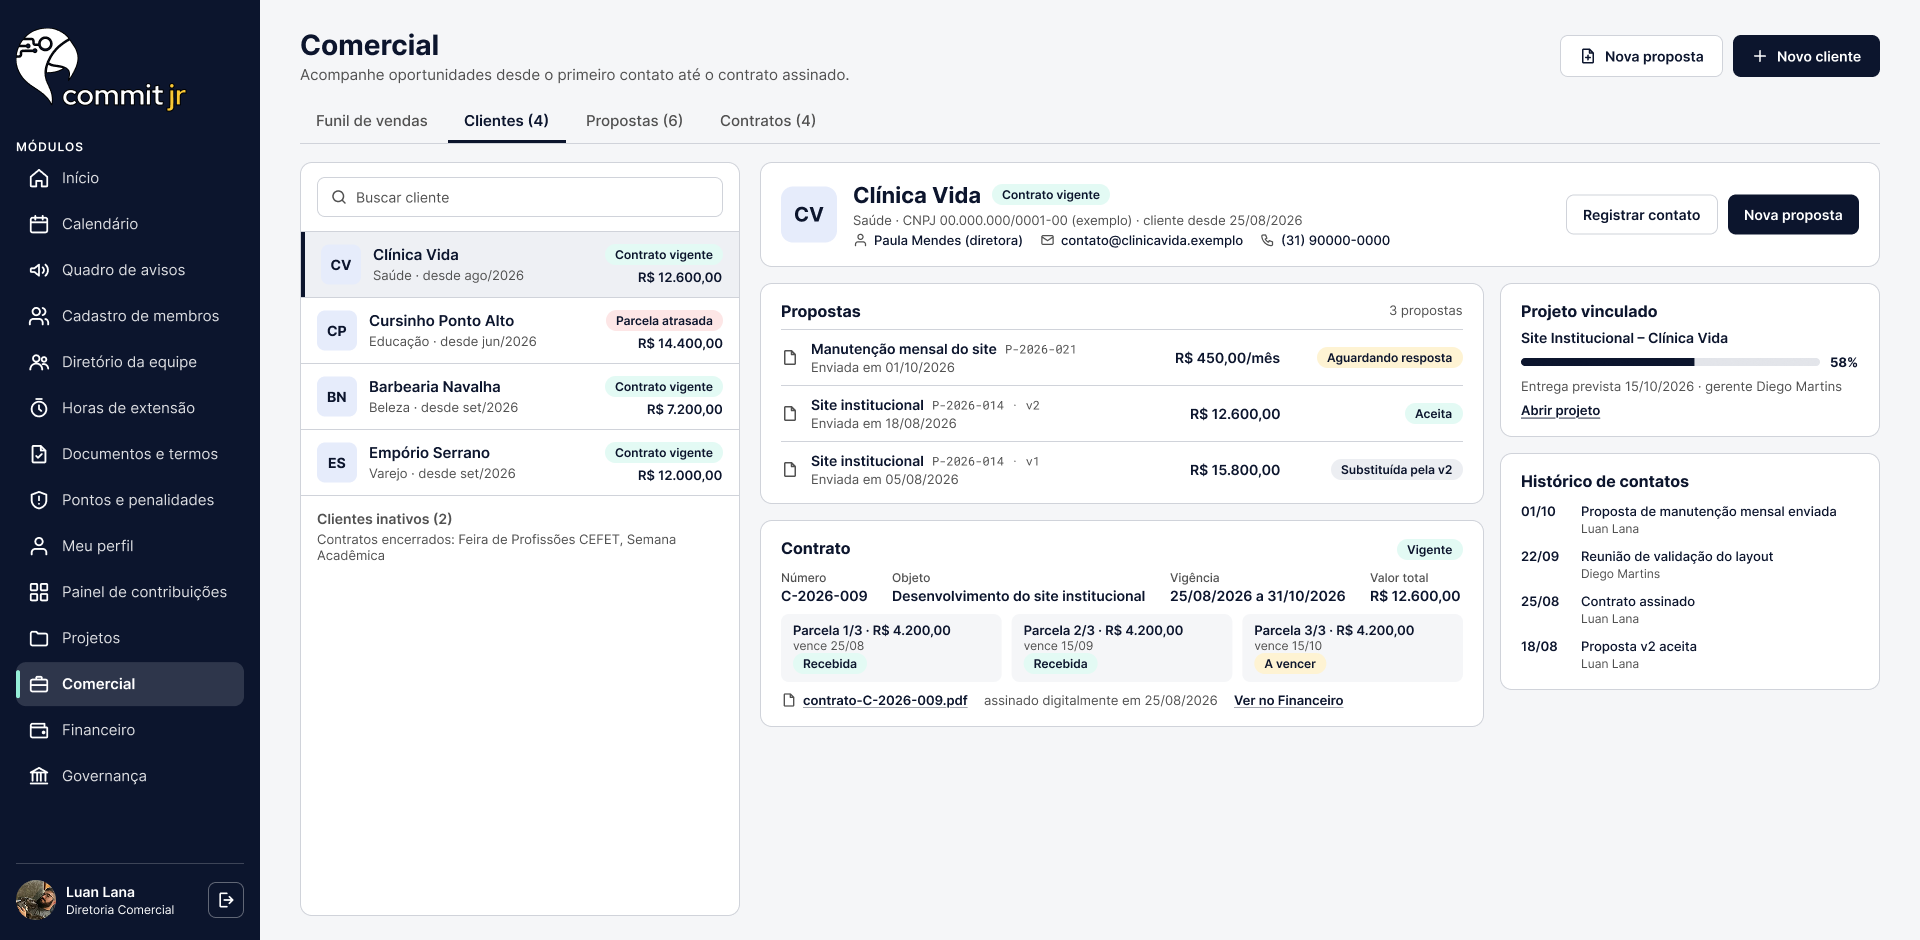
\includegraphics[width=0.88\textwidth]{Telas/comercial-clientes}} \\
\hline
\end{tabular}
\end{center}

\begin{center}
\begin{tabular}{|p{2.0cm}|p{11.5cm}|}
\hline
\textbf{PT-032} & \textbf{Comercial -- Funil de Vendas (UC-16)} \\
\hline
\multicolumn{2}{|c|}{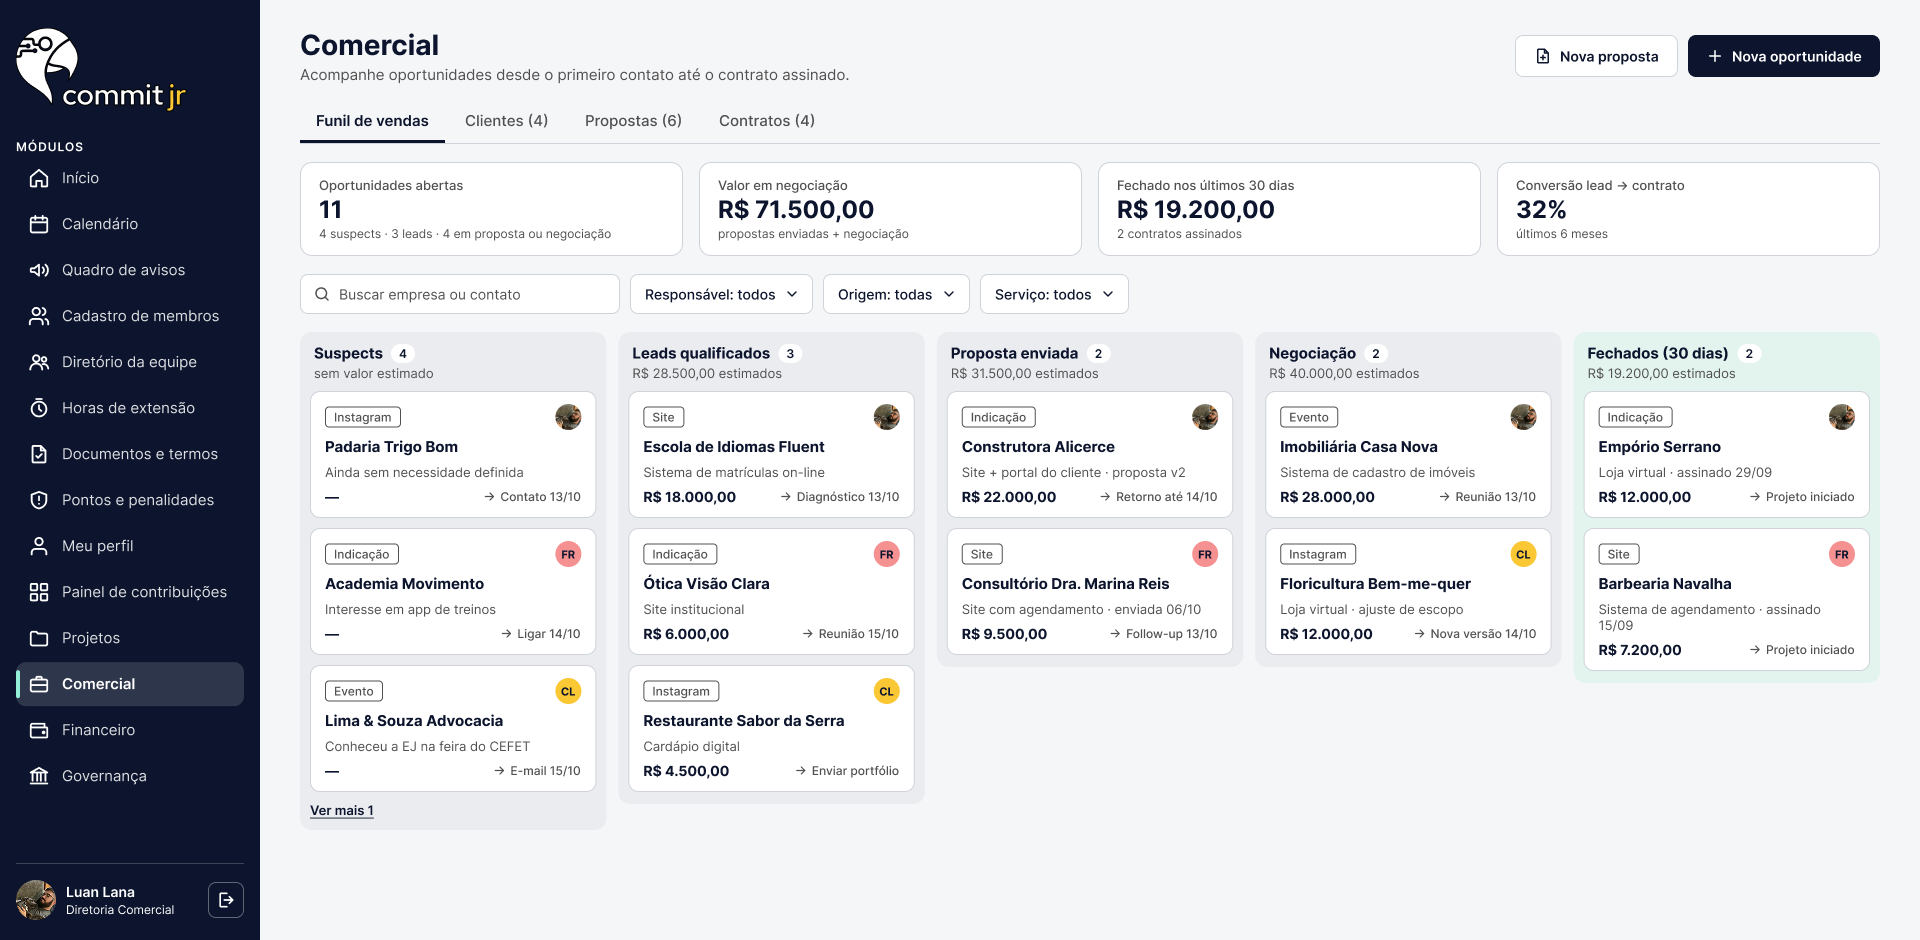
\includegraphics[width=0.88\textwidth]{Telas/comercial-funil-vendas}} \\
\hline
\end{tabular}
\end{center}

\begin{center}
\begin{tabular}{|p{2.0cm}|p{11.5cm}|}
\hline
\textbf{PT-033} & \textbf{Financeiro -- Visão Geral e Aprovações Pendentes (UC-20, UC-21)} \\
\hline
\multicolumn{2}{|c|}{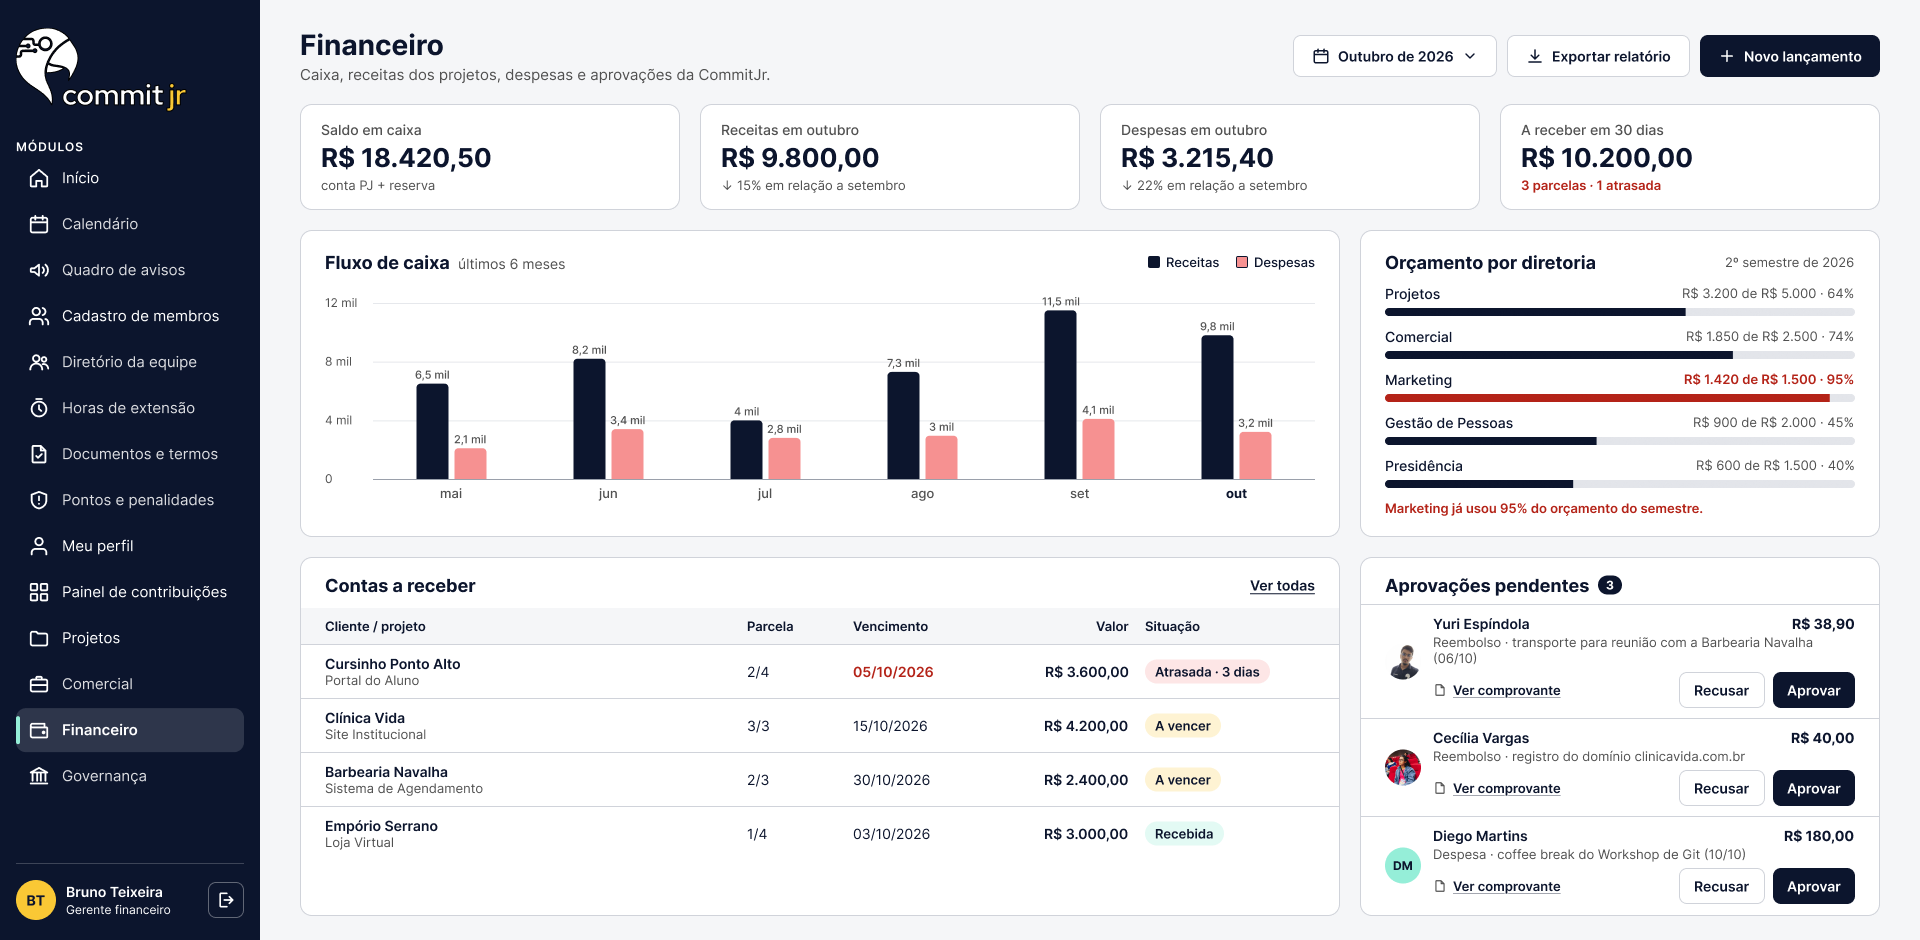
\includegraphics[width=0.88\textwidth]{Telas/financeiro-visao-geral}} \\
\hline
\end{tabular}
\end{center}

\begin{center}
\begin{tabular}{|p{2.0cm}|p{11.5cm}|}
\hline
\textbf{PT-034} & \textbf{Financeiro -- Novo Lançamento de Entrada (UC-20)} \\
\hline
\multicolumn{2}{|c|}{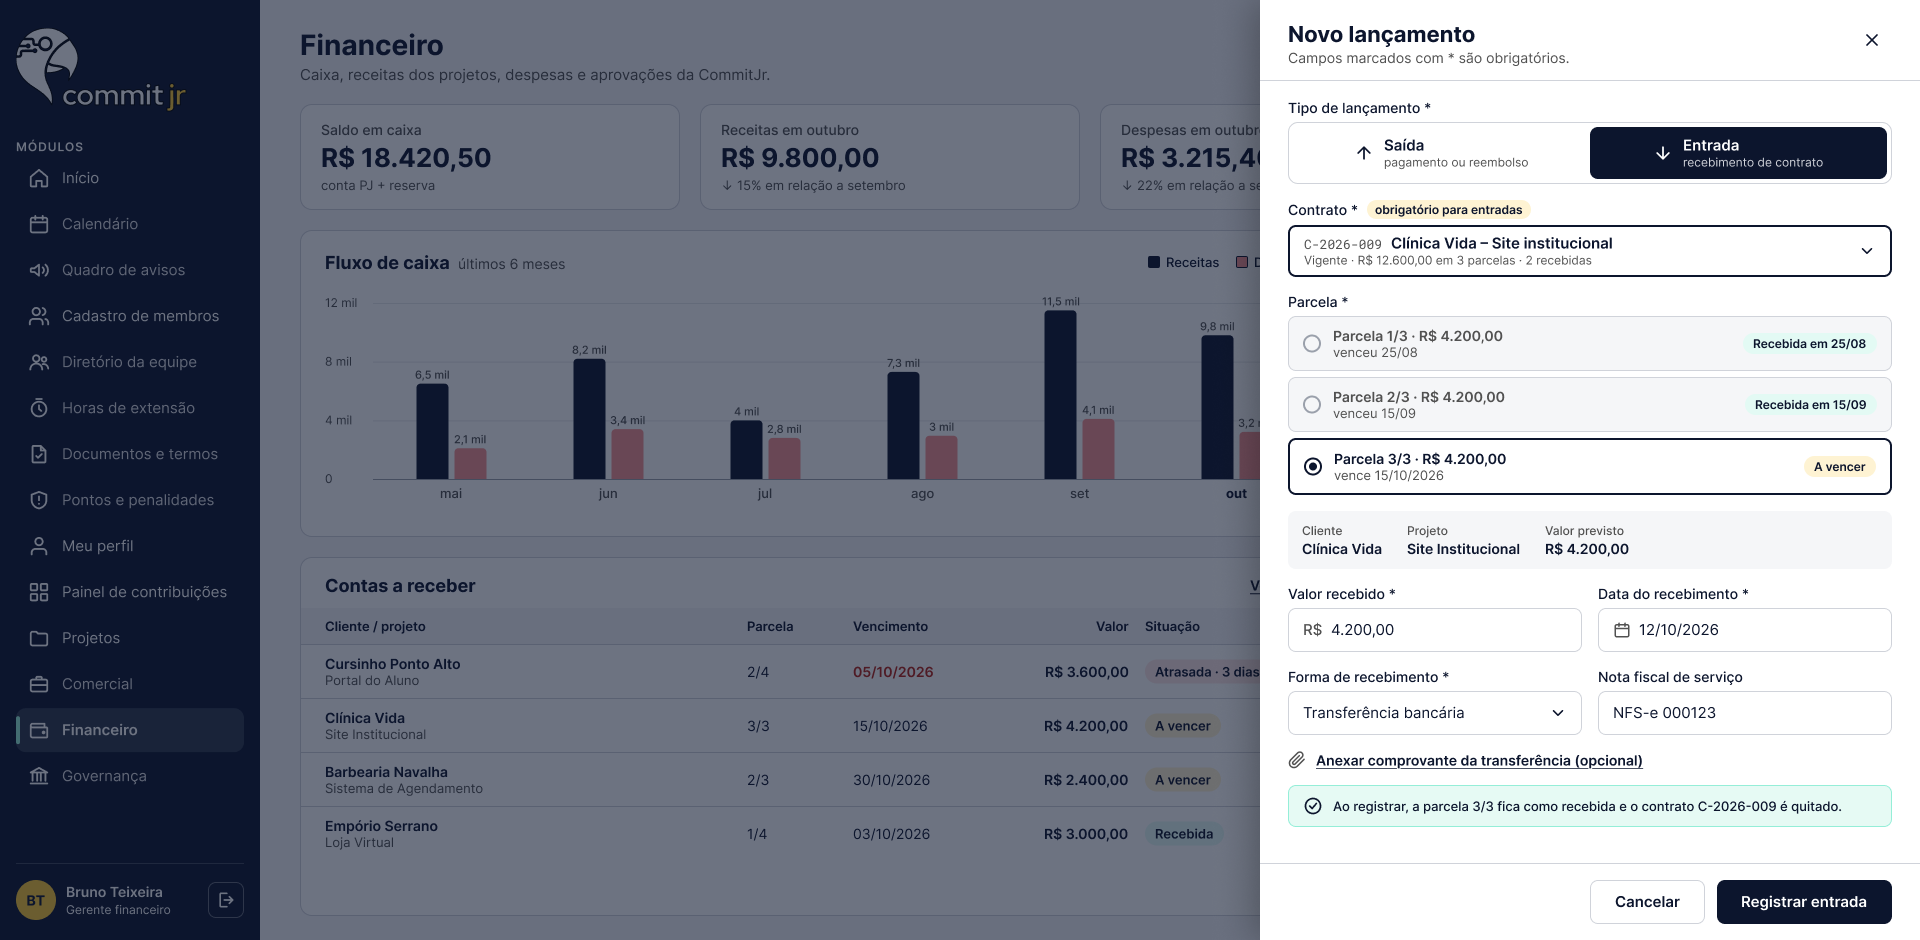
\includegraphics[width=0.88\textwidth]{Telas/financeiro-lancamento-entrada}} \\
\hline
\end{tabular}
\end{center}

\begin{center}
\begin{tabular}{|p{2.0cm}|p{11.5cm}|}
\hline
\textbf{PT-035} & \textbf{Financeiro -- Novo Lançamento de Saída (UC-20)} \\
\hline
\multicolumn{2}{|c|}{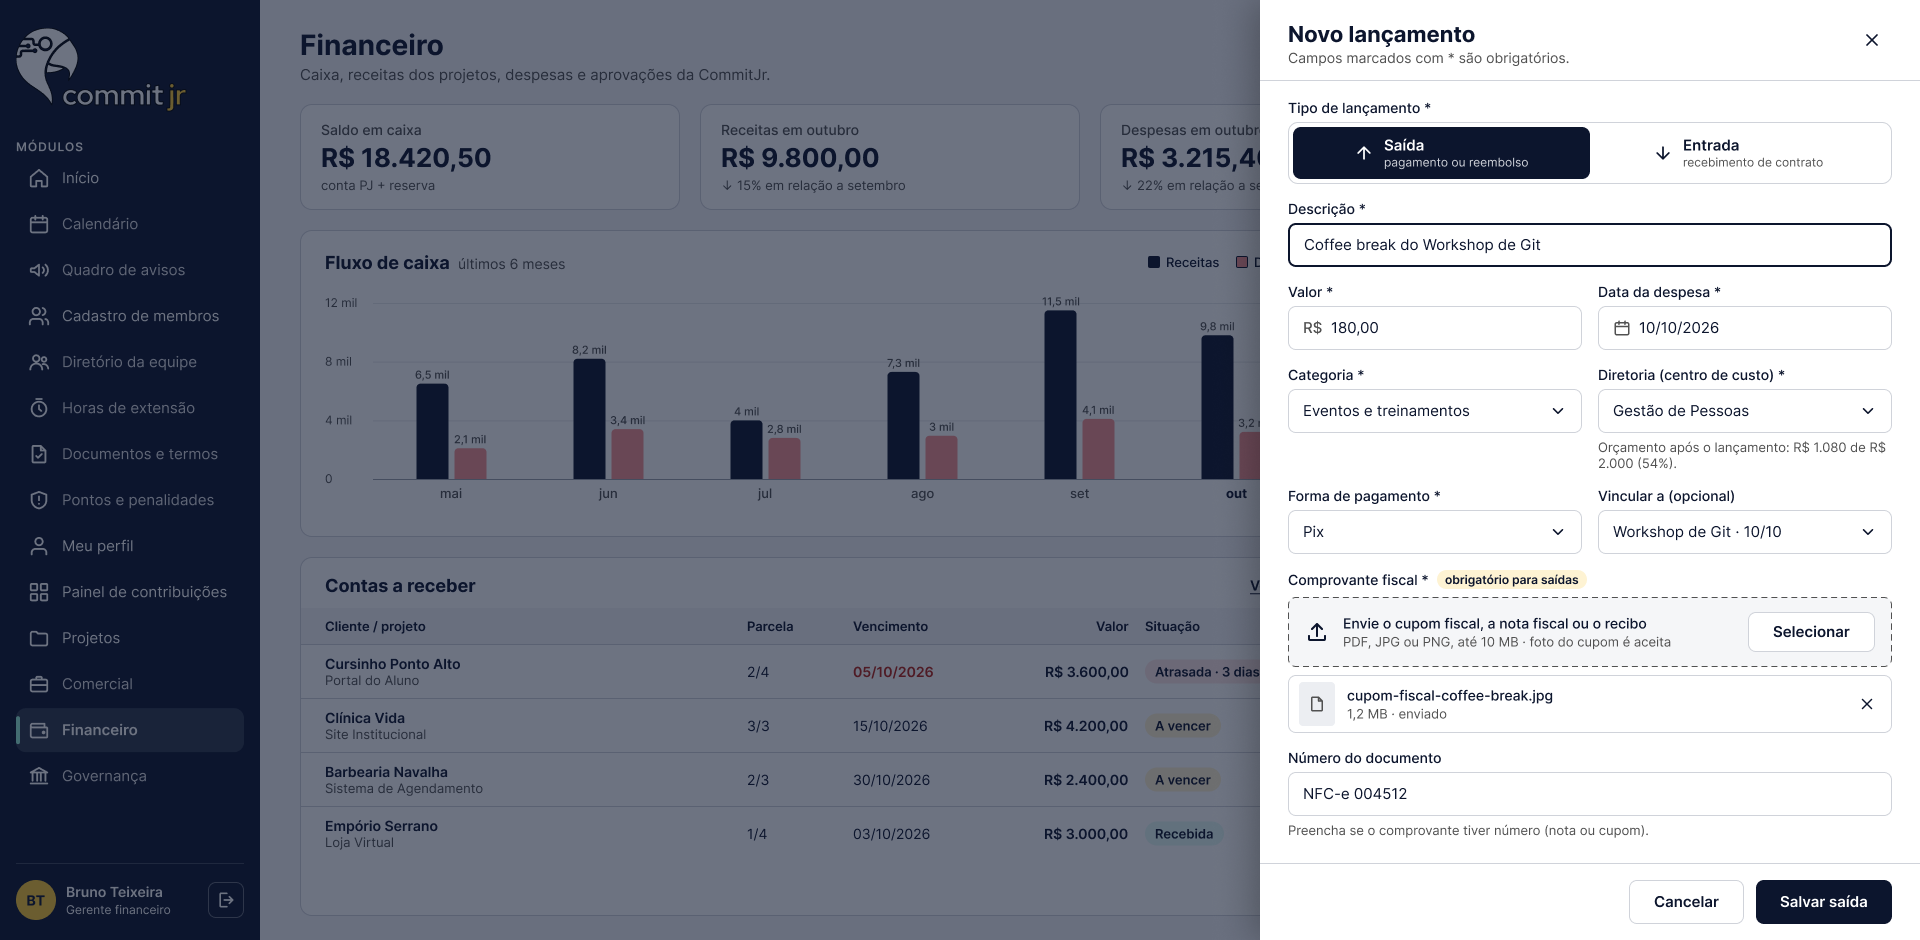
\includegraphics[width=0.88\textwidth]{Telas/financeiro-lancamento-saida}} \\
\hline
\end{tabular}
\end{center}

\clearpage
